\documentclass[12pt,a4paper]{amsart}
% ukazi za delo s slovenscino -- izberi kodiranje, ki ti ustreza
\usepackage[slovene]{babel}
%\usepackage[cp1250]{inputenc}
%\usepackage[T1]{fontenc}
\usepackage[utf8]{inputenc}
\usepackage{amsmath,amssymb,amsfonts}
\usepackage{url}
%\usepackage[normalem]{ulem}
\usepackage[dvipsnames,usenames]{color}
\usepackage{array}
\usepackage[pdftex]{graphicx}

% ne spreminjaj podatkov, ki vplivajo na obliko strani
\textwidth 15cm
\textheight 24cm
\oddsidemargin.5cm
\evensidemargin.5cm
\topmargin-5mm
\addtolength{\footskip}{10pt}
\pagestyle{plain}
%\overfullrule=15pt % oznaci predlogo vrstico
\overfullrule=0pt


% ukazi za matematicna okolja
\theoremstyle{definition} % tekst napisan pokoncno
\newtheorem{definicija}{Definicija}[section]
\newtheorem{primer}[definicija]{Primer}
\newtheorem{opomba}[definicija]{Opomba}

\renewcommand\endprimer{\hfill$\diamondsuit$}


\theoremstyle{plain} % tekst napisan posevno
\newtheorem{lema}[definicija]{Lema}
\newtheorem{izrek}[definicija]{Izrek}
\newtheorem{trditev}[definicija]{Trditev}
\newtheorem{posledica}[definicija]{Posledica}


% za stevilske mnozice uporabi naslednje simbole
\newcommand{\R}{\mathbb R}
\newcommand{\N}{\mathbb N}
\newcommand{\Z}{\mathbb Z}
\newcommand{\C}{\mathbb C}
\newcommand{\Q}{\mathbb Q}

% ukaz za slovarsko geslo
\newlength{\odstavek}
\setlength{\odstavek}{\parindent}
\newcommand{\geslo}[2]{\noindent\textbf{#1}\hspace*{3mm}\hangindent=\parindent\hangafter=1 #2}

% naslednje ukaze ustrezno popravi
\newcommand{\program}{Finančna matematika} % ime studijskega programa: Matematika/Finan"cna matematika
\newcommand{\imeavtorja}{Metod Jazbec} % ime avtorja
\newcommand{\imementorja}{doc. dr. Aljoša Peperko} % akademski naziv in ime mentorja
\newcommand{\naslovdela}{Splošna definicija diferencirane zasebnosti}
\newcommand{\letnica}{2018} %letnica diplome


% vstavi svoje definicije ...




\begin{document}

% od tod do povzetka ne spreminjaj nicesar
\thispagestyle{empty}
\noindent{\large
UNIVERZA V LJUBLJANI\\[1mm]
FAKULTETA ZA MATEMATIKO IN FIZIKO\\[5mm]
\program\ -- 1.~stopnja}
\vfill

\begin{center}{\large
\imeavtorja\\[2mm]
{\bf \naslovdela}\\[10mm]
Delo diplomskega seminarja\\[1cm]
Mentor: \imementorja}
\end{center}
\vfill

\noindent{\large
Ljubljana, \letnica}
\pagebreak

\thispagestyle{empty}
\tableofcontents
\pagebreak

\thispagestyle{empty}
\begin{center}
{\bf \naslovdela}\\[3mm]
{\sc Povzetek}
\end{center}
% tekst povzetka v slovenscini
V delu predstavimo diferencirano zasebnost. Gre za matematično definicijo zasebnosti pri javni objavi ter rudarjenju podatkov. Predstavljena je splošna definicija v kontekstu metričnih prostorov in verjetnostne mere, ki omogoča enotno obravnavo različnih vrst podatkov. Pokažemo nekaj osnovnih izrekov, ki omilijo zahteve definicije. Obravnavan je Laplacov mehanizem za numerične podatke. Podana je izpeljava spodnjih mej za največjo napako zasebnih odzivnih mehanizmov. V nadaljevanju se osredotočimo na funkcijske podatke. S pomočjo teorije Gaussovih procesov in Hilbertovih prostorov z reprodukcijskim jedrom pokažemo uporabo diferencirane zasebnosti na primeru jedrne cenilke gostote. Osnovne mehanizme implementiramo in predstavimo rezultate.
\vfill
\begin{center}
{\bf General definition of differential privacy}\\[3mm] % prevod slovenskega naslova dela 
{\sc Abstract}
\end{center}
% tekst povzetka v anglescini
We introduce the concept of differential privacy, mathematical definition for privacy preserving data publishing and data mining. General definition in context of metric spaces and probability measure is given. Further, we present some theorems which help to alleviate the requirements of described definition. Laplace mechanism for numerical data and lower bounds on errors of response mechanisms are presented. We later turn focus to functional data. Using Gaussian process and Reproducing Kernel Hilbert Spaces we present how differential privacy is used for privatization of density kernel estimator. Most of the described mechanism are also implemented and results are presented at the end.

\vfill\noindent
{\bf Math. Subj. Class. (2010):} 97R50, 94A15  \\[1mm]  
{\bf Ključne besede:} diferencirana zasebnost, odzivni mehanizem, metrični prostor, funkcijski podatki, verjetnostna mera  \\[1mm]  
{\bf Keywords:} differential privacy, response mechanism, metric space, functional data, probability measure
\pagebreak



% tu se zacne tekst seminarja
\section{Uvod}
Dandanes živimo v dobi podatkov. Podjetja ter ustanove zbirajo podatke o svojih uporabnikih in jih nato uporabijo za izboljšanje algoritmov oz. tehnologije. Posledično postaja vse bolj pomembno  vprašanje  varovanja podatkov. Kako omogočiti strokovnjakom in inženirjem dostop do velikih podatkovnih baz, hkrati pa ohraniti zasebnost posameznikov? Kako lahko podjetja uporabijo vse podatke, ki jih zbirajo o svojih uporabnikih, ne da bi s tem ogrozili njihove zasebnosti? Obstaja veliko različnih pristopov (najbolj pogoste so t. i. metode anonimizacije), vendar se je izkazalo, da je veliko od teh neprimernih in so izpostavljeni raznim napadom. Posebej velja izpostaviti napad s pomočjo pomožne baze (angl. background/auxiliary attack), pri katerem napadalec uporabi dodatno podatkovno bazo za razkritje identite posameznikov v prvotni bazi (znan primer Netflix [12]).  V ta namen se je v zadnjih 15 letih pojavil koncept diferencirane zasebnosti, ki postavlja vprašanje varovanja podatkov v okvir matematične teorije.  Osnovna ideja je, da se odgovor na poizvedbo ne bo spremenil, če podatki o enem konkretnem posamezniku so ali niso v bazi. To dosežemo prek vnosa `naključnosti' v podatkovno bazo; odgovori na poizvedbe niso več deterministični, ampak so probabilistični. Na ta način omogočimo dostop do globalnih lastnosti celotne populacije, zaščitimo pa konkretne informacije o posameznikih. Mnogi vidijo diferencirano zasebnost kot odlično rešitev, uporabljajo jo podjetja kot so Apple in Uber [3,4]. Na drugi strani obstaja precej kritik. Ena glavnih izmed njih je, da koncept diferencirane zasebnosti sicer ponuja lepe matematične in teoretične temelje, ni pa zares uporaben v praksi. 
\newline
\newline
Pomembno je razumevanje, da se diferencirana zasebnost ne ukvarja z zaščito podatkov samih. Tako ne ponuja odgovora na problem, kako podatke varno shraniti na nekem serverju (da jih zaščitimo pred hekerskemi vdori ipd.). Ukvarja se s tem, kako ohraniti zasebnost pri procesu objavljanja (angl. data publishing) in pridobivanja podatkov (angl. data mining). Za lažje razumevanje pred nadaljevanjem navedimo še dva primera. Prvi se je zgodil leta 2000, ko ameriške bolnišnice niso zaščitile javno dostopnih podatkov na primeren način. Uporabili so prej omenjene metode anonimizacije, kar pomeni, da so iz podatkov odstranili vse eksplicitne identifikatorje (ime, emšo). Podatki so tako vsebovali le npr. spol pacienta, rojstni datum, poštno številko in zdravstveno stanje (poenostavljen primer). Izkazalo se je, da lahko te podatke združimo (angl. cross-reference) s podatki iz volilnega sistema, in na ta način razkrijemo identiteto pacientov v prvotni podatkovni bazi. En možen način za rešitev tega problema bi bil, da bolnišnice sploh ne bi javno objavile podatkov, ampak bi dostop do podatkovne baze raziskovalcem omogočile le prek dovoljenih poizvedb. Znanstveniki bi lahko tako 'vprašali' koliko odstotkov oseb ženskega spola ima določeno bolezen, ne bi pa smeli povprašati po diagnozi konkretnega posameznika. Pri takem pristopu se naravno pojavi vprašanje, točno katere poizvedbe dovolimo. Po eni strani izbire nočemo preveč omejiti (znanstvenikom želimo omogočiti kvalitetne podatke), po drugi strani ne želimo razkriti preveč informacij o posamezniku. Hkrati se tudi izkaže, da lahko v primeru determinističnih poizvedb napadalec samo na podlagi odgovorov na poizvedbe sklepa o lastnostnih posameznika. Ponazorimo to s preprostim zgledom na podatkih iz tabele 1. Recimo, da bi napadalec rad izvedel Edijevo diagnozo. Privzemimo, da ima na voljo poizvedbo $Q_i$, ki kot odgovor vrne vsoto prvih i vrstic. Dodatno tudi ve, da se Edi nahaja na 5. mestu v tabeli. Tako bi lahko izvedel poizvedbi $Q_4$ in $Q_5$ in iz razlike obeh sklepal, da Edi ima diabetes.  Odgovor na to problematiko ponuja diferencirana zasebnost, pri kateri poizvedbe postanejo probabilistične in napadalec kljub dodatnim informacijam ne more priti do gotovih sklepov o Edijevi diagnozi.
\begin{table}
\begin{center}
 \begin{tabular}{| c | c |} 
 \hline
 \textbf{Pacient} & \textbf{Diabetes}  \\ [0.5ex] 
 \hline
 Anja & 1  \\ 
 \hline
 Bojan & 1\\
 \hline
 Cene & 0 \\
 \hline
 Darja & 0  \\
 \hline
 Edi & 1  \\  
 \hline
\end{tabular}
\caption{Podatkovna baza z imeni pacientov in podatki o diabetesu.}
\end{center}
\end{table}
\newline
\newline
Drugi primer, ki je danes zelo aktualen, se pojavi pri procesu rudarjenja podatkov. Podjetja za izboljšanje svoje programske opreme beležijo skoraj vsako potezo svojih uporabnikov na pametnih telefonih ali računalnikih. Te podatke potem uporabijo za razvoj sistemov, kot so priporočanje vsebin in pomoč pri tipkanju (angl. auto-correct). Vsi ti algoritmi za delovanje potrebujejo ogromne količine učnih primerov. Uporabnikom je tako rečeno, da morajo žrtvovati del zasebnosti za izboljšanje tehnologije, ki jo uporabljajo. Diferencirana zasebnost ponuja možnost, da temu ni tako (če se izkaže, da je skalabilna). Tak pristop že uporablja Apple [3], ki nekatere podatke še preden jih iz naprave (npr. iz iphona) pošlje na centralni server, zaščiti s pomočjo algoritmov, ki slonijo na diferencirani zasebnosti. 
\newline
\newline
V prvem delu diplomske naloge se posvetimo teoretičnemu ozadju. V praksi imamo opravka z različnimi vrstami podatkov, v literaturi pa se diferencirana zasebnost pogosto definira le za posamezno vrsto podatkov. Predstavili bomo model, ki omogoča, da se koncept diferencirane zasebnosti definira v splošnem, tj. za vse vrste podatkov hkrati. V nadaljevanju bo podanih tudi nekaj osnovnih teoretičnih rezultatov, ki izhajajo iz tega modela. V drugem delu se posebej osredotočimo na funkcijske podatke in nazadnje večino obravnavanih mehanizmov še implementiramo ter opišemo rezultate.

\section{Matematična priprava}

Naj bo $\Omega$ neprazna množica s pripadajočo algebro $\mathcal{S}$. Označimo s $\sigma(\mathcal{S})$ najmanjšo $\sigma$-algebro, ki vsebuje $\mathcal{S}$ (rečemo da $\mathcal{S}$ generira $\sigma(\mathcal{S})$).
\begin{definicija}
Monoton razred $\mathcal{M}$ je družina podmnožic $\Omega$ (torej $\mathcal{M} \subset \mathcal{P(\mathcal{M})}$) z naslednjima lastnostima:
\begin{itemize}
\item  $\{A_i\}_{i=1,...\infty} \in \mathcal{M}, A_i \subseteq A_{i+1} \Rightarrow \bigcup_{i=1,...\infty} A_i \in \mathcal{M}$ (zaprtost za monotono naraščajoče števne unije),
\item  $\{A_i\}_{i=1,...\infty} \in \mathcal{M}, A_i \supseteq A_{i+1} \Rightarrow \bigcap_{i=1,...\infty} A_i \in \mathcal{M}$ (zaprtost za monotono padajoče števne preseke).
\end{itemize}
\end{definicija}
Iz definicije takoj sledi, da je vsaka $\sigma$-algebra monoton razred (uporabimo zaprtost za poljubne števne unije in preseke). Naslednji izrek karakterizira $\sigma(\mathcal{S})$ kot najmanjši monoton razred, ki vsebuje algebro $\mathcal{S}$.

\begin{izrek} Naj bo $\mathcal{S}$ algebra in $\mathcal{M}$ monoton razred na množici $\Omega$. Naj velja še $\mathcal{S} \subseteq \mathcal{M}$. Potem sledi $\sigma{(\mathcal{S})} \subseteq \mathcal{M}$.
\end{izrek}
\proof
 Označimo z $m(\mathcal{S})$ najmanjši monoton razred, ki vsebuje $\mathcal{S}$ (dobimo ga kot presek vseh monotonih razredov na $\Omega$, ki vsebujejo $\mathcal{S}).$ Ker za vsak $\mathcal{M}$ z lastnostjo $\mathcal{S} \subseteq \mathcal{M}$ velja $m(\mathcal{S}) \subseteq \mathcal{M}$, vidimo, da je dovolj pokazati $\sigma(\mathcal{S}) \subseteq m(\mathcal{S})$. Za dokaz tega je dovolj pokazati, da je $m(\mathcal{S}) $ $\sigma$-algebra (sledi iz dejstva, da je $\sigma(\mathcal{S})$ najmanjša $\sigma$-algebra, ki vsebuje $\mathcal{S}$). Ker je $m(\mathcal{S})$ monoton razred, je dovolj pokazati, da je $m(\mathcal{S})$ algebra. Algebra je $\sigma$-algebra namreč natanko tedaj, ko je monoton razred \footnote{Netrivialna je tu samo zaprtost za števne unije pri prehodu iz monotonega razreda na $\sigma$-algebro: naj bo $\mathcal{A}$ algebra in monoton razred. Za vsak $A_n \in \mathcal{A}$ definirajmo $B_k:=\cup_{n=1}^k A_n \in \mathcal{A}$, Potem $B_k$ tvorijo naraščajoče zaporedje in iz zaprtosti za monotone unije monotonih razredov dobimo $\cup_{k=1}^\infty B_k=\cup_{n=1}^\infty A_n \in \mathcal{A}$. Sledi, da je $\mathcal{A}$ $\sigma$-algebra.}.
\newline
Pokažimo najprej zaprtost za komplemente. Obravnavajmo družino množic $\mathcal{G} = \{ A\hspace{0.1cm}|\hspace{0.1cm} A^c \in m(\mathcal{S})\}$.  Ker je $m(\mathcal{S})$ monoton razred, sledi da je tudi $\mathcal{G}$. Dodatno velja še $\mathcal{S} \subseteq \mathcal{G}$ (sledi iz $\mathcal{S} \subseteq m(\mathcal{S})$ in dejstva, da je $\mathcal{S}$ algebra, torej zaprta za komplement). To nam zagotovi $m(\mathcal{S}) \subseteq \mathcal{G}$, s čimer smo pokazali, da je $m(\mathcal{S})$ zaprt za komplemente.
\newline
Pokažimo še zaprtost za končne unije. Definirajmo družino množic $\mathcal{H}_1 = \{ A\hspace{0.1cm}|\hspace{0.1cm} A \cup B \in m(\mathcal{S}), \forall B \in \mathcal{S}\}$. Potem je $\mathcal{H}_1$ monoton razred in $\mathcal{S} \subseteq \mathcal{H}_1$. Iz minimalnosti sledi $m(\mathcal{S}) \subseteq \mathcal{H}_1$. Definirajmo še  $\mathcal{H}_2 = \{ B\hspace{0.1cm}|\hspace{0.1cm} A \cup B \in m(\mathcal{S}), \forall A \in m(\mathcal{S})\}$. Spet velja, da je $\mathcal{H}_2$ monoton razred. Ker je $m(\mathcal{S}) \subseteq \mathcal{H}_1$, sledi da $A \in m(\mathcal{S})$ in $B \in \mathcal{S}$ skupaj implicirata $A \cup B \in m(\mathcal{S})$. Povedano drugače, $B \in S$ implicira $B \in \mathcal{H}_2$. Torej je $\mathcal{S} \subseteq \mathcal{H}_2$  in iz minimalnosti dobimo $m(\mathcal{S}) \subseteq \mathcal{H}_2$, iz česar sledi, da $A,B \in m(\mathcal{S})$ implicira $A \cup B \in m(\mathcal{S})$. Torej je $m(\mathcal{S})$ res algebra in izrek je dokazan.
\qed
\newline
\newline
Na kratko ponovimo še nekaj osnovnih pojmov o metričnih prostorih.
\begin{itemize}
\item Metrični prostor $(D, \rho)$ je \textit{končen} (angl. finite), če ima končno število elementov/točk (torej $|D| < \infty$). Primer je množica hobijev v primeru 3.1.
\item Metrični prostor $(D, \rho)$ je \textit{končno-dimenzionalen} (angl. finite-dimensional), če ima končno bazo. Primer je $\mathbb{R}^n$.
\item Metrični prostor $(D, \rho)$ je \textit{neskončno-dimenzionalen} (angl. infinite-dimensional), če nima končne baze. Primer je $C([0,1])$.
\end{itemize}
\begin{definicija}
Metrični prostor $(D, \rho)$ je \textit{kompakten}, če ima vsako zaporedje v $D$ konvergetno podzaporedje z limito prav tako v $D$ (povedano drugače, vsako zaporedje v $D$ ima vsaj eno stekališče vsebovano v $D$).
\end{definicija}
\begin{opomba}
Zgoraj podana definicija ne opisuje najbolj splošnega pojma kompaktnosti, ampak gre za  t. i. kompaktnost glede na zaporedja (angl. sequentially compactness), kar zadostuje za potrebe tega diplomskega dela. Oba pojma kompaktnosti sta namreč ekvivalentna v primeru metričnih prostorov. Se pa pojma razlikujeta, če delamo s topološkimi prostori (kompaktnost tu definiramo drugače, prek pokritij in podpokritij).
\end{opomba}
V primeru ko je $D \subset \mathbb{R}^n$ (podmnožica Evklidskega prostora), dodatno vemo, da je D kompakten natanko tedaj, ko je zaprt in omejen.
\begin{lema}
Naj bo $(D, \rho)$ končen metričen prostor. Potem je $D$ kompakten.
\end{lema}
\proof
Vzemimo poljubno zaporedje v $D$ z neskočno mnogo elementi. Vidimo, da se mora vsaj en element iz $D$ v zaporedju pojaviti neskončno mnogokrat. V nasprotnem primeru zaporedje ne bi imelo neskončno mnogo elementov (sledi iz končnosti $D$). Ponavljajoče se vrednosti tega elementa tvorijo podzaporedje, ki je seveda konvergentno. Torej je po zgornji definiciji $D$ kompakten.
\qed
\newline
\newline
Definirajmo še metriko $\rho_H$, t.i. \textit{Hammingovo razdaljo}, ki jo bomo potrebovali za izpeljavo nekaterih nadaljnjih rezultatov. 
\begin{definicija}
Naj bo $D$ poljubna množica in $a , b \in D^n$. Potem je  \textit{Hammingova razdalja} $\rho_H(a,b)$ enaka številu mest, na katerih se vektorja $a$ in $b$ razlikujeta.
\end{definicija}
Opazimo, da je v eno-dimenzionalnem primeru  ta metrika ekvivalentna diskretni. Morda se bralcu zastavi vprašanje, kako deluje taka metrika na vektorju npr. funkcij. Če želimo enakost skoraj povsod, lahko za $D$ vzamemo prostor $L^2$, torej primerjamo med seboj ekvivalenčne razrede funkcij.  Hammingova metrika na prvi pogled tudi ni najbolj uporabna, saj pove le, ali sta elementa danega metričnega prostora različna in ne 'koliko' sta različna. Zanimivo je, da je to v primeru diferencirane zasebnosti primerna stvar, saj tu med sabo primerjamo podatkovne baze in ne vnosov znotraj posamezne baze. 
\newline
\newline
V zadnjem poglavju bomo za izpeljavo nekaterih rezultatov potrebovali še osnovno teorijo jedrnih funkcij v statistični analizi, Gaussovih procesov ter Hilbertovih prostorov z reprodukcijskim jedrom. Z namenom večje preglednosti navedemo še izrek Radon-Nikodym.
\begin{definicija}
Funkcija $K$ je jedrna funkcija (angl. kernel function), če je nenegativna, integrabilna ter slika v prostor realnih števil.
\end{definicija}
\begin{opomba}
Zgoraj podana definicija je najbolj splošna, ponavadi pa zahtevamo še dva dodatna pogoja in sicer simetričnost, torej $K(x) = K(-x)$, ter normalizacijo
$$
\int_{-\infty}^{\infty} K(u)du=1.
$$
Enostaven primer je eno-dimenzionalno Gaussovo jedro, ki ima obliko $K(u)=\frac{1}{\sqrt{2\pi}}e^{-\frac{u^2}{2}}$ (vidimo, da gre kar za gostoto standarno normalne porazdelitve).
\end{opomba}
\begin{definicija}
Gaussov proces, parametriziran z indeksno množico $T$, je slučajni proces $\{X_t : t \in T\}$, za katerega velja, da je za vsak končni nabor točk $t_1,...,t_n \in T$ slučajni vektor
$$
(X_{t_1},...,X_{t_n})
$$
porazdeljen multivariatno normalno.
\end{definicija}
\begin{opomba}
Gaussov proces je kot slučajni proces definiran na nekem verjetnostnem prostoru  $(\Omega, \mathcal{F}, \mathbb{P})$. Pri fiksnem $\omega \in \Omega$ je preslikava $T \rightarrow \mathbb{R}$ (oz. $t \rightarrow X_t(\omega)$) realizacija ali trajektorija Gaussovega procesa $X_t$. Gaussov proces je popolnoma določen s funkcijama povprečja  in kovariance: 
$$m(t) = \mathbb{E}X_t, \quad K(s,t) = Cov(X_s,X_t).$$
\end{opomba}

Spomnimo se, da je Hilbertov prostor $\mathcal{H}$ poln metrični prostor (vsako Cauchyjevo zaporedje ima limito vsebovano v tem prostoru), kjer je metrika podana prek skalarnega produkta, torej za $f,g \in \mathcal{H}$ velja $d(f,g) = \sqrt{<f-g,f-g>}$.
\begin{definicija}
Naj bo $H$ Hilbertov prostor, katerega elementi so funkcije oblike $f: X \rightarrow \mathbb{R}$ (pri tem je $X$ poljubna množica). Označimo z $L_x$ linearen funkcional, ki vsako funkcijo $f \in \mathcal{H}$ izvrednoti v x, torej $$L_x : f \rightarrow f(x).$$ Potem je $\mathcal{H}$ Hilbertov prostor z reprodukcijskim jedrom natanko tedaj, ko je $L_x$ zvezen operator nad $\mathcal{H}$ za vsak $x \in X$. 
\end{definicija}
\begin{opomba}
Opišimo podano definicijo ter reprodukcijsko lastnost na še bolj intiutiven način. Z uporabo Rieszovega reprezentacijskega izreka o funkcionalih opazimo, da za vsak $x \in X$ obstaja natanko en $K_x \in \mathcal{H}$ z lastnostjo
$$
f(x) = L_x(f) = \langle f, K_x \rangle_{\mathcal{H}}, \quad \forall f \in \mathcal{H}.
$$
Če sedaj namesto $f$ vzamemo $K_x \in \mathcal{H}$, sledi, da za vsak $y \in X$ obstaja $K_y \in \mathcal{H}$, da velja
$$
K_x(y) = L_y(K_x) = \langle K_y, K_x \rangle_{\mathcal{H}}.
$$
To nam omogoča, da definiramo reprodukcijsko jedro Hilbertovega prostora $\mathcal{H}$ kot funckijo $K: X \times X \rightarrow \mathbb{R}$, kjer je $K(x,y)=\langle K_y, K_x \rangle_{\mathcal{H}}.$
\newline
\newline
Alternativno si lahko Hilbertov prostor $\mathcal{H}$ predstavljamo kot zaprtje linearne ogrinjače funckij oblike $K_x, x \in X$. Za dve funkciji oblike $f = \sum_{i=1}^{n}\theta_i K_{x_i}$ in $ g = \sum_{j=1}^{m}\xi_j K_{y_j}$ ($\xi_i, \theta_i \in \mathbb{R} \; \forall i, \; x_1,...,x_n,y_1,...,y_m \in X$) ima tako njun skalarani produkt obliko
$$
\langle f, g\rangle_{\mathcal{H}} = \sum_{i=1}^{n}\sum_{j=1}^{m}\theta_i \xi_j K(x_i,y_j).
$$
\end{opomba}
\begin{definicija} 
Naj bosta $\mu$ in $\nu$ meri definirani na istem merljivem prostoru $(X, \Sigma)$. Rečemo, da je $\mu$ absolutno zvezna glede ne $\nu$ (tudi da $\nu$ dominira $\mu$), če velja $\mu(A) = 0$ za vse merljive množice $A$, za katere velja $\nu(A)=0$. Označimo $\mu \ll \nu$.
\end{definicija}

\begin{izrek} [Radon-Nikodym]
Naj bosta $\mu$ in $\nu$ meri definirani na istem merljivem prostoru $(X, \Sigma)$. Dodatno naj velja, da sta $\mu$ in $\nu$ $\sigma$-končni meri. Če velja  $\mu \ll \nu$, potem obstaja merlijva funkcija $f : X \rightarrow [0,\infty)$, da za vsako merljivo množico $A \subseteq X$ velja
\begin{gather*}
\mu(A) = \int_A f d \nu = \int_A \frac{d \mu}{d \nu} d \nu
\end{gather*}
Funkcija f se imenuje Radon-Nikodymjev odvod.
\end{izrek}



\begin{opomba}
V verjetnosti je gostota slučajne spremenljivke $X$ s porazdelitvenim zakonom $F_X$ ravno Radon-Nikodymjev odvod inducirane mere $dF_X$ glede na neko osnovno mero (v primeru zveznih slučajnih spremenljivk ponavadi vzamemo Lebesgueovo mero $\lambda$, torej dobimo $f=\frac{dF_X}{d \lambda}$). Včasih rečemo, da je slučajna spremenljivka $X$ absolutno zvezna, če ima gostoto (v Radon-Nikodymjevem smislu).
\end{opomba}

\section{Splošni podatkovni model in definicija diferencirane zasebnosti}

\subsection{Predstavitev podatkovne baze}
Naj bo $(U, \rho)$ poljuben metrični prostor in $D \subseteq U$. Posamezni vnosi v opazovani podatkovni bazi so elementi množice $D$. Celotno bazo prikažemo z vektorjem \textbf{d} $= (d_{1}, ..., d_{n}) \in D^n$, kjer $d_{i} \in D$ predstavlja i-ti vnos oz. vrstico. 
\newline
\newline
Množico $U$ opremimo z Borelovo $\sigma$-algebro (označimo jo z $\mathcal{A}_{U}$), ki je najmanjša $\sigma$-algebra, ki vsebuje vse odprte množice v $U$. Tako $\sigma$-algebro generiramo preko metrične topologije. Za lažjo predstavo podajmo grob opis tega postopka. S pomočjo metrike $\rho$ na $U$ lahko definiramo odprte krogle  $B_{r}(x) = \{y \in U\hspace{0.1cm}|\hspace{0.1cm}\rho(x,y) < r\}$. To zadošča, da lahko definiramo bazo topologije, ki je oblike $\mathcal{B} = \{B_{r}(x)\hspace{0.1cm}|\hspace{0.1cm}x \in U, r>0\}$ (povedano drugače, vsak metrični prostor je hkrati topološki prostor oz. metrika nam porodi topologijo). Ko enkrat imamo topologijo  (gre za podmnožico potenčne množice $U$, ki vsebuje vse odprte množice v $U$), lahko le-to uporabimo za generiranje Borelove $\sigma$-algebre.
\newline
\newline
$\mathcal{A}_{U}$ nam potem naravno porodi $\mathcal{A}_{D} := \{A \in \mathcal{A}_{U} | A \subset D \}$ na $D$. Predpostavimo tudi, da je $U^n$ (in s tem $D^n$) opremljen s produktno $\sigma$-algebro, ki je najmanjša $\sigma$-algebra, ki vsebuje $\{A_{1} \times ... \times A_{n} | A_{i} \in \mathcal{A}_{U}\}$ in jo označimo z $\mathcal{A}_{U^n}$. 
\newline
\newline
Tak model podatkovne baze je splošen ($U$ je namreč poljubni metrični prostor) in nam omogoča enotno obravnavo različnih vrst podatkov: numeričnih, kategoričnih in funkcijskih.
\begin{primer}  
Recimo, da imamo na voljo podatkovno bazo, v kateri so zabeleženi hobiji posameznikov. Množico vseh hobijev lahko označimo s $\mathcal{H}=\{nogomet, kitara,...\}$. Predpostavka o končnosti $\mathcal{H}$ je tu smiselna in neomejujoča. Za $D$ potem lahko vzamemo $2^\mathcal{H}$. Pri izbiri metriki imamo precej proste roke, vzemimo npr. diskretno metriko  $\rho(A,B)=1$ če $A \neq B$ in 0 drugače. Borelova $\sigma$-algebra $\mathcal{A}_{D}$ je tu enaka $2^{2^{\mathcal{H}}}$. Opazimo tudi, da ni nujno, da imajo vsi elementi v $D^n$ (torej vnosi v naši podatkovni bazi) enako število elementov, kar odraža dejstvo, da nimamo vsi ljudje enakega števila hobijev.
\end{primer}

\begin{primer} Kot primer za numerične podatke obravnavajmo barvne slike, torej $D = \mathbb{R}^{n\times m \times 3}$ (RGB\footnote{RGB je kratica, ki prihaja iz angleščine in pomeni `red', `green' in `blue'. Opisuje barvni model, ki je pogost pri analizi barvnih slik.}  slike dimenzije $n \times m)$. Kot metrika se tu naravno ponuja $\rho(A,B)=\sum_{i,j,k}  |a_{i,j,k}-b_{i,j,k}|$. Za Borelovo $\sigma$-algebro $\mathcal{A}_{D}$  vzamemo produktno $\sigma$-algebro, torej  $\mathcal{A}_{D}=\sigma(\{A_{1} \times A_{2} \times A_{3} | A_{1} \in \mathcal{B}(\mathbb{R}^n),  A_{2} \in \mathcal{B}(\mathbb{R}^m),  A_{3} \in \mathcal{B}(\mathbb{R}^3) \})$. Ta koncept lahko razširimo na 3-D barvne slike in tudi na video posnetke.
\end{primer}

\begin{primer} Primer mešanih podatkov nam ponuja enostavna baza zdravstvenih podatkov. Recimo, da so elementi naše baze oblike \textit{(kvazi-identifikator pacienta, starost, spol, bolezen, bolezen 1, bolezen 2, ...)}. $D$ potem lahko izberemo takole 

\begin{gather*}
D=\{1,2,...,st. pacientov\} \times \{1,...,120\} \times \{M,F\} \times \\
\{Ljubljana, ... , Spodnji Duplek\} \times \{0,1\}^n.
\end{gather*}
Kar pogosto naredimo v praksi je, da najprej kategorične podatke spremenimo v numerične (npr. z uporabo `one-hot' kodiranja\footnote{Pristop v programiranju s katerim stolpec v podatkovni bazi, ki vsebuje diskretne podatke, spremenimo v več numeričnih stolpcev, ki vsebujejo le ničle ter enke.}). Metrika na $D$ in pripadajoča Borelova algebra potem izgledata podobno kot v prejšnjem primeru.
\end{primer}

\begin{primer}
Navedimo še primer, ko imamo opravka s t. i. funkcijskimi podatki. Ti se pojavijo npr. pri merjenju porabe elektrike v gospodinjstvih, kar lahko predstavimo kot graf porabe v odvisnosti od časa. Če meritev opravimo le ob določenih časovnih točkah, lahko za $D$ vzamemo npr. prostor zaporedij (angl. sequence space) $l_{\infty}$ ali $l_{2}$. Drugače lahko vzamemo za $D$ npr. $C([0,T])$ ali $L_{2}([0,T])$. Tu T označuje dolžino opazovanega časovnega obdobja. Dodajmo še, da so prostori $l_p$ le posebni primeri prostorov $L_p$, ko delamo na merljivem prostoru $(\mathbb{N}, 2^\mathbb{N})$, za mero pa vzamemo t. i. mero štetja. Vsi ti prostori so Banachovi prostori (t.j. polni normirani prostori), kar pomeni, da imajo naravno podano normo. Le-ta nam inducira metriko $\rho$, prav tako pa lahko prek norme pridemo do pripadajoče Borelove $\sigma$-algebre (glej izpeljavo zgoraj prek metrične topologije). 
\end{primer}
\newline
\newline
Pravimo da sta dve podatkovni bazi, \textbf{d}$= (a_{1},...,a_{n})$ in $\textbf{d'}= (b_{1},...,b_{n})$,  \textit{sosednji}, če se razlikujeta v natanko enem vnosu. Torej:
\begin{itemize}
\item obstaja $j\in\{1,...n\}$, da velja $a_{j} \neq b_{j}$,
\item za vsak $i\in\{1,...,n\} \setminus j$ velja $a_{i} = b_{i}$.
\end{itemize}
Sosednji bazi označimo z \textbf{d} $\sim$ \textbf{d\'}. Če obravnamo $D^n$ kot metrični prostor s pripadajočo Hammingovo metriko $\rho_{H}$, je \textbf{d} $\sim$ \textbf{d\'} natanko tedaj, ko je $\rho_{H}$(\textbf{d},\textbf{d\'})$=1$.
\newline
\newline
Za izpeljavo nekaterih rezultatov v nadaljevanju moramo predpostaviti, da je $D$ kompakten metrični prostor. V primeru kompaktnosti definiramo še diameter kot $diam(D) := \max\limits_{d,d' \in D}\rho(d,d')$. Obstoj maksimuma v tej definiciji je posledica dejstva, da zvezna funkcija $\rho$ doseže svoj maksimum na kompaktni množici $D$.

\subsection{Modeliranje poizvedb}
Poizvedba (angl. query) je način pridobitve željenih informacij iz podatkovne baze. V prejšnjem poglavju smo podatkovno bazo predstavili kot metrični prostor in enako sedaj storimo za množico vseh možnih odgovor (angl. set of all possible responses) na posamezno poizvedbo. Tak metrični prostor označimo z $(E_{Q}, \rho_{Q})$ in ga ponovno opremimo z Borelovo $\sigma$-algebro $\mathcal{A}_{Q}$ (indeks Q tu ponazarja odvisnost od poizvedbe, kar je naravno, saj različne poizvedbe vodijo do različnih množic možnih odgovorov). Sedaj lahko definiramo poizvedbo kot merljivo funkcijo $Q: U^n \rightarrow E_{Q} $, torej $Q^{-1}(A) \in \mathcal{A}_{U^n}$ za vsako $A \in \mathcal{A}_Q$.
\begin{primer} Kot pri konstrukciji podatkovne baze \textbf{d} $\in D^n$, imamo tudi pri izbiri prostora možnih odgovorov precej proste roke. Če se vrnemo na primer podatkovne baze hobijev, bi npr. lahko povprašali po številu ljudi, ki igrajo nogomet. Odgovor na to poizvedbo bi bil numeričen ($E_{Q} = \mathbb{N}$). Lahko pa bi nas zanimalo, kateri so 3 najpogostejši hobiji v bazi. Odgovor tu bi bil verjetno množica hobijev  ($E_{Q} = 2^\mathcal{H}$).
\end{primer}
\newline
\newline
Dalje lahko definiramo \textit{odzivni mehanizem} (angl. response mechanism).. 
\begin{definicija}
Naj bo $(\Omega , \mathcal{F}, \mathbb {P} )$ verjetnostni prostor, $\textbf{d}\in D^n$ opazovana podatkovna baza in $\mathcal{Q}(n)$ (n se nanaša na dimenzijo podatkovne baze) množica (možnih oz. dovoljenih) poizvedb. \textit{Odzivni mehanizem} (za izbran nabor poizvedb $\mathcal{Q}(n)$) je definiran kot družina slučajnih spremenljivk
\begin{equation}\label{odzivni}
 \{X_{Q,\textbf{d}} : \Omega \rightarrow  E_{Q} | Q \in  \mathcal{Q} (n), \textbf{d} \in D^n\} \tag{1}.
\end{equation} 
\end{definicija}

Pričakovana napaka takega mehanizma za dano poizvedbo $Q$ in podatkovno bazo \textbf{d} je dana z $\mathbb{E}[\rho_{Q}(X_{Q,\textbf{d}},Q(\textbf{d})]$. 
V nadaljevanju bo pogosto navedeno $\mathbb{P}(X_{Q,\textbf{d}} \in A)$, kar je seveda okrajšava za $\mathbb{P}(\{\omega \in \Omega : X_{Q,\textbf{d}}(\omega) \in A \})$.
\newline
\newline
Ločimo dva glavna primera odzivnih mehanizmov:
\begin{itemize}
\item \textit{Perturbacija podatkovne baze} (angl. sanitised response mechanism). Tu vnesemo naključnost v podatke, še preden podamo odgovor na poizvedbo. Za to potrebujemo družino merljivih preslikav (slučajnih vektorjev) $\{ Y_{\textbf{d}}: \Omega \rightarrow U^n | \textbf{d} \in D^n\}$ Če taka družina obstaja, ima odzivni mehanizem obliko kompozituma
\begin{equation}\label{odzivni2}
 X_{Q,\textbf{d}} = Q \circ Y_{\textbf{d}}. \tag{2}
\end{equation} 
V praksi se ponavadi to izvede prek t. i. dodajanja šuma, torej $Y_{\textbf{d}} = \textbf{d}+N$, kjer je $N$ slučajni vektor v $U^n$. Za tak pristop je potrebno, da ima $U^n$ primerno algebraično obliko (npr. vektorski prostor ali monoid, kar nam zagotovi zaprtost za seštevanje).
\item \textit{Perturbacija odgovorov na poizvedbo} (angl. output perturbation). Kot sklepamo že iz imena, tokrat podatke perturbiramo šele po poizvedbi. Recimo, da imamo podano poizvedbo $Q: U^n \rightarrow E_{Q}$. V primeru da obstaja družina merljivih preslikav $ \{Z_{q}:\Omega \rightarrow E_{Q} | q  \in E_{Q} \}$, je odzivni mehanizem definiran kot
\begin{equation}\label{odzivni3}
X_{Q,\textbf{d}}=Z_{Q(\textbf{d})}.\tag{3}
\end{equation} 
\end{itemize}

\subsection{Definicija diferencirane zasebnosti}
Sedaj smo pripravili vse potrebno in lahko definiramo pojem diferencirane zasebnosti.

\begin{definicija}{\textbf{Diferencirana zasebnost za posamezno poizvedbo}}
Naj bo $\epsilon \geq 0$ in $0 \leq \delta \leq 1 $. Odzivni mehanizem je $(\epsilon, \delta)$-diferencirano zaseben za poizvedbo $Q$, če za vse $\textbf{d} \sim \textbf{d'} \in D^n$  in za vse $A\in\mathcal{A}_{Q}$ velja 
\begin{equation}\label{diferen}
\mathbb{P}(X_{Q,\textbf{d}} \in A) \leq e^\epsilon \mathbb{P}(X_{Q,\textbf{d'}} \in A) + \delta \tag{4}
\end{equation}
\end{definicija}
\begin{opomba} 
\begin{itemize}
\item Vidimo, da je diferencirana zasebnost koncept, ki se tiče odzivnega mehanizma. Ideja zadaj je, da se odgovor na naš mehanizem ne sme preveč razlikovati za dve sosednji bazi (drugače povedano, če en posamezen vnos je ali ni v bazi, to ne bo preveč vplivalo na rezultat mehanizma). Na ta način diferencirano zasebni mehanizmi preprečujejo, da bi lahko prišli do sklepov o konkretnih posameznikih. 
\item Zasebnost opisujemo s parametroma $\epsilon$ in $\delta$. Na začetku se je uporabljal samo $\epsilon$ ( t. i. stroga diferencirana zasebnost), vendar se je izkazalo, da je tako oblika pogosto preveč zahtevna za implementacijo v praksi. $\delta$ tako zajema verjetnost, da se osnovni mehanizem `zlomi'. Nižja kot bosta oba parametra, večja bo zasebnost, a bo hkrati posledična manjša natančnost (bolj bodo odgovori na poizvedbe oddaljeni od resničnih).  Gre za kompromis med zasebnostjo in natančnostjo (angl. trade-off between accuracy and privacy).
\item Pomembna je tudi \textit{simetričnost} definicije. Neenakost mora veljati, tudi če zamenjamo vlogi \textbf{d} in \textbf{d'}.
\end{itemize}
\end{opomba}

\begin{primer}
Za boljše razumevanje ponazorimo definicijo s primerom. Za dano poizvedbo $Q$ izberimo konkretni sosednji bazi \textbf{d}, \textbf{d'} $\in D^n$ in $A\in \mathcal{A}_{Q}$. Označimo $a = \mathbb{P}(X_{Q,\textbf{d}}\in A)$ in $b = \mathbb{P}(X_{Q,\textbf{d'}}\in A)$. Zaradi simetričnosti morata v primeru $(\epsilon, \delta)$-diferencirane zasebnosti mehanizma, veljati obe neenakosti, torej $a \leq e^{\epsilon}b+\delta$ in $b \leq e^{\epsilon}a+\delta$. Obravnavajmo dva primera:
\begin{itemize}
\item $a=b$ : Enakost obeh verjetnosti kaže na to, da se odgovor na poizvedbo ni spremenil z dodajanjem oz. odstranitvijo posameznika iz baze. Obe neenakosti tu sledita trivialno.
\item $a>b$ (brez škode za splošnost, zaradi simetričnosti nam ni treba obravnavati še primera $a<b$) : nenakost $b \leq e^{\epsilon}a+\delta$ tu prav tako sledi trivialno, druga neenakost pa nam podaja mejo, za koliko je lahko verjetnost b manjša od a, da bo obravnavani mehanizem še vedno diferencirano zaseben. V primeru $(\epsilon, \delta) = (0.05, 0.05)$, mehanizem, pri katerem bo za dan $A \in \mathcal{A}_{Q}$ $\; a=0.9$ in $b=0.8$, ne bo diferencirano zaseben, saj $0.9 \nleq e^{0.05} 0.8 + 0.05 \doteq 0.89$ (ni izpolnjena druga neenakost).
\end{itemize}
Ta primer nakazuje  zahtevnost testiranja $(\epsilon, \delta)$-diferencirane zasebnosti mehanizma.Zzgornji postopek moramo namreč ponoviti za vse sosednje baze v $D^n$ in za vse elemente $A$ Borelove $\sigma$-algebra $\mathcal{A}_Q$ (teh je pogosto neštevno mnogo)! V praksi je to seveda v večini primerov neizvedljivo. V nadaljevanju bo podanih nekaj rezultatov, ki dane zahteve omilijo.
\end{primer}


\begin{definicija} {\textbf{Diferencirana zasebnost}}
Odzivni mehanizem je $(\epsilon, \delta)$-diferencirano zaseben glede na $\mathcal{Q}(n)$ (množica poizvedb), če je $(\epsilon, \delta)$-diferencirano zaseben za vsako poizvedbo $Q \in \mathcal{Q}(n)$
\end{definicija}

\section{Omilitev zahtev definicije diferencirane zasebnosti}
\subsection{Zadostne testne množice}
V prejšnjem poglavju smo definirali koncept diferencirane zasebnosti in izpostavili nekatere omejitve. Ena izmed njih je bila, da je potrebno pogoj iz definicije \eqref{diferen} preveriti za vse elemente $\mathcal{A}_Q$ ($\sigma$-algebra množice možnih odgovorov na dano poizvedbo $Q$). Naslednji izrek nam pove, da je dovolj, da pogoj (4) preverimo le za vse elemente algebre $\mathcal{S}$, ki $\mathcal{A}_Q$ generira.

\begin{izrek}
 Naj bosta podana odzivni mehanizem \eqref{odzivni} in poizvedba $(E_Q, \mathcal{A}_Q, Q)$. Naj bo $\mathcal{S} \subset \mathcal{A}_Q$ algebra in naj velja $\sigma(\mathcal{S}) = \mathcal{A}_Q$. Če \eqref{diferen} velja za vse $A \in \mathcal{S}$, potem velja za vse $A \in \mathcal{A}_Q$. 
\end{izrek}
\proof 
Označimo z $\mathcal{B} \subset \mathcal{P}(E_Q) $ vse množice za katere je pogoj \eqref{diferen} izpolnjen. Po predpostavki iz izreka velja $\mathcal{S} \subseteq \mathcal{B}$. Naj bo $A_1 \subseteq A_2 \subseteq ... $, kjer je $A_i \in \mathcal{B}$ za vsak $i \in \mathbb{N}$, poljubno monotono naraščajoče zaporedje množic v $\mathcal{B}$. Naj bosta še \textbf{d}, \textbf{d'} $\in D^n$ poljubni sosednji podatkovni bazi. Potem velja 
\begin{gather*}
\mathbb{P}(X_{Q,\textbf{d}} \in \bigcup_{i} A_i) = \lim_{i \to\ \infty} \mathbb{P}(X_{Q,\textbf{d}} \in A_i)  \leq \\
\leq  e^\epsilon\lim_{i \to\ \infty} \mathbb{P}(X_{Q,\textbf{d'}} \in A_i) + \delta = \\
=  e^\epsilon \mathbb{P}(X_{Q,\textbf{d'}} \in \bigcup_{i} A_i) + \delta
\end{gather*}
kjer smo pri obeh enakostih uporabili zveznost verjetnostne mere, pri neenakosti pa dejstvo, da za vsak i velja $A_i \in \mathcal{B}$. Identičen argument pokaže, da enako velja za monotono padajoča zaporedja množic v $\mathcal{B}$. S tem smo pokazali, da je $\mathcal{B}$ monoton razred. Iz tega in iz dejstva, da je $\mathcal{S} \subseteq \mathcal{B}$ (po uporabi izreka 2.2  o monotonih razredih), sledi, da je tudi $\sigma(\mathcal{S}) = \mathcal{A}_Q \subseteq \mathcal{B}$.
\qed
\newline
\begin{primer}
Uporabimo zgornji izrek na konkretnem zgledu. Vzemimo poizvedbo $Q$ z $E_Q = C([0,1])$, torej zavzema vrednosti v prostoru zveznih funkcij. Kot normo vzemimo $||f||_\infty = sup\{|f(t)| : t \in [0,1]\}$ in pripadajočo Borelovo $\sigma$-algebro $\mathcal{A}_Q$. Naj bo podan še odzivni mehanizem $X_{Q,\textbf{d}}$. $X_{Q,\textbf{d}}(\omega)$ torej leži v $C([0,1])$ za vsak $\omega \in \Omega$.
\newline
Izberimo še $k \in \mathbb{N}$ in k-terico realnih števil $0 \leq t_1 \leq \ldots \leq t_k \leq 1$ in definirajmo preslikavo $ \pi _{t_1,\ldots,t_k}: C([0,1]) \rightarrow \mathbb{R}^k$ kot $$\pi _{t_1,\ldots,t_k}(f) = (f(t_1),\ldots,f(t_2)).$$ Te preslikave so merljive (natančneje $(\mathcal{A}_Q, \mathcal{B}(\mathbb{R}^k))$ merljive) in zato lahko definiramo $X_{Q,\textbf{d}}^{t_1,\ldots,t_k} = \pi _{t_1,\ldots,t_k} \circ X_{Q,\textbf{d}}$. Opazimo, da je sedaj $X_{Q,\textbf{d}}^{t_1,\ldots,t_k} (\omega) \in \mathbb{R}^k$ za vsak $\omega \in \Omega$. Pokažimo, da če je končno-dimenzionalen mehanizem $X_{Q,\textbf{d}}^{t_1,\ldots,t_k}$ diferencirano zaseben glede na definicijo $\eqref{diferen}$ za vsak $k$ in za vse k-terice $0 \leq t_1 \leq \ldots \leq t_k \leq 1$, potem je tudi $X_{Q,\textbf{d}}$ diferencirano zaseben. Najprej opazimo, da iz naše predpostavke sledi, da so opazovani mehanizmi zasebni za množice oblike $A = \pi _{t_1,\ldots,t_k}^{-1}(B)$, kjer je $B$ Borelova množica v $\mathbb{R}^k$: 
\begin{gather*}
\mathbb{P}(X_{Q,\textbf{d}} \in A) =  \mathbb{P}(X_{Q,\textbf{d}} \in \pi _{t_1,\ldots,t_k}^{-1}(B)) = \mathbb{P}(X_{Q,\textbf{d}}^{t_1,\ldots,t_k} \in B) \leq \\
 \leq e^{\epsilon}\mathbb{P}(X_{Q,\textbf{d'}}^{t_1,\ldots,t_k} \in B) + \delta = e^{\epsilon}\mathbb{P}(X_{Q,\textbf{d'}} \in A) + \delta, \quad \forall \textbf{d} \sim \textbf{d'} \in D^n
\end{gather*}


Množice A tvorijo algebro na $C([0,1])$ (posledica lastnosti praslik). Označimo to algebro z 
$$\mathcal{F}_0 = \bigcup_{\substack{B \in \mathcal{B}(\mathbb{R}^k), \\ |\{t_1,...,t_k\}| < \infty}} \pi _{t_1,\ldots,t_k}^{-1}(B).$$

 Izkaže se, da je $\sigma$-algebra, ki jo te množice generirajo, kar Borelova $\sigma$-algebra na $C([0,1])$ (glej izrek 7.2.1 v [9]). Torej dobimo $\sigma({\mathcal{F}_0}) = \mathcal{A}_Q$ in po uporabi zgornjega izreka sledi rezultat.
\end{primer}

\subsection{Identična poizvedba v primeru perturbacije podatkovne baze}
Identična poizvedba je, kot pove že ime, poizvedba, ki ne spremeni podatkovne baze. Odgovor na tako poizvedbo je torej celotna podatkovna baza. Lahko bi rekli, da je identična poizvedba enaka javni objavi podatkov. Označimo jo z $ I_n : D^n \rightarrow D^n$, $\;I_n$(\textbf{d})=\textbf{d}. 
\newline
\newline
Ponavadi imamo opravka s sistemom, ki podpira več kot eno možno poizvedbo v podatkovno bazo. V tem primeru moramo pogoj diferencirane zasebnosti preveriti za vsako izmed razpoložljivih poizvedb posebej. Naslednji izrek pokaže, da je za mehanizme, ki perturbirajo podatkovno bazo \eqref{odzivni2}, dovolj ta pogoj preveriti le za identično poizvedbo.
\begin{izrek} 
Naj bo odzivni mehanizem s perturbacijo podatkovne baze  $(\epsilon , \delta)$-diferencirano zaseben glede na identično poizvedbo $(U^n, \mathcal{A}_{U^n}, I_n)$. Potem sledi, da je tak mehanizem $(\epsilon , \delta)$-diferencirano zaseben glede na katerokoli poizvedbo $(E_Q, \mathcal{A}_Q, Q)$.
\end{izrek}
\begin{opomba} Velja poudariti pomembnost tega, da v izreku ne postavimo nobenih omejitev na množico možnih odgovorov $E_Q$.  Lahko bi bili naši podatki zelo enostavni, npr. naravna števila $D \in \mathbb{N}$, odgovori na poizvedbo pa bi bile funkcije ali zaporedja, tj. npr. $E_Q = C([0,1])$ ali $E_Q = l_\infty$. Zgornji izrek nam omogoči, da v tem primeru namesto da preverjamo pogoj \eqref{diferen} za vse elemente $\sigma$-algebre $C([0,1])$, moramo pogoj preveriti le za vse elemente $\sigma$-algebre $2^{\mathbb{N}}$, kar je občutno lažje in lahko predstavlja razliko med v praksi izvedljivo in neizvedljivo nalogo.
\end{opomba}
\proof 
Naj bosta \textbf{d}, \textbf{d'} $\in D^n$ poljubni sosednji podatkovni bazi. Po predpostavki velja 
\begin{equation}\label{star}
\mathbb{P}(Y_{\textbf{d}} \in E) \leq e^\epsilon \mathbb{P}(Y_{\textbf{d'}} \in E) + \delta \tag {*}
\end{equation}
za vsak $E \in \mathcal{A}_{U^n}$. Vzemimo sedaj poljubno poizvedbo $(E_Q, \mathcal{A}_Q, Q)$. Ker je $Q: U^n \rightarrow E_Q$ merljiva, velja  $Q^{-1}(A)\in \mathcal{A}_{U^n}$ za vsak $A \in \mathcal{A}_Q$. Potem z uporabo \eqref{star} sledi 
\begin{gather*}
\mathbb{P}(X_{Q, \textbf{d}} \in A) = \mathbb{P}(Q(Y_{ \textbf{d}}) \in A)  \\ = \mathbb{P}(Y_{\textbf{d}} \in Q^{-1}(A)) 
\leq e^\epsilon \mathbb{P}(Y_{\textbf{d'}} \in Q^{-1}(A)) + \delta \\ 
= \mathbb{P}(Q(Y_\textbf{d'}) \in A) + \delta = \mathbb{P}(X_{Q,\textbf{d'}} \in A) + \delta
\end{gather*}
in vidimo, da je dan mehanizem diferenciano zaseben tudi za poljubno izbrano poizvedbo $Q$.
\qed
\newline
\newline
Sedaj lahko izpostavimo pomembno razliko med prej omenjenima vrstama odzivnih mehanizmov, perturbacija podatkovne baze \eqref{odzivni2} in perturbacija odgovorov na poizvedbe \eqref{odzivni3}. Pri slednjem načinu gre ponavadi za to, da najprej izvedemo poizvedbo, šele na to pa prek dodajanja šuma zaščitimo podatke. V tem primeru obstaja možnost, da bi napadalec večkrat izvedel identično poizvedbo in bi nato prek povprečja prišel do prave vrednosti iskanih podatkov. Posledično moramo omejiti število možnih poizvedb (oz. vrsto poizvedb, tj. prepovedati npr. identično poizvedbo). V primeru \eqref{odzivni2} tak napad ni mogoč, saj tu še preden podamo odgovor na poizvedbo zaščitimo podatke s primernim diferencirano zasebnim mehanizom. Odgovor na identično poizvedbo je tako vedno enak in napadalec ne more priti do sklepov o pravi vrednosti podatkov v bazi. 
\begin{primer}
Ponazorimo zgoraj povedano še na konkretnem primeru, ki je koristen tudi za boljše razumevanje formalizma opisanega modela ter razlike med posameznimi vrstami odzivnih mehanizmov. Recimo, da poizvedbo $Q$ ponovimo k-krat ($ k \geq 1$). To lahko modeliramo kot eno samo poizvedbo $Q^{(k)}: U^n \rightarrow E_{Q}^{(k)}$, kjer $E_{Q}^{(k)} = E_Q \times ... \times E_Q$. Torej je $Q^{(k)}(\textbf{d}) = (Q(\textbf{d}), ... , Q(\textbf{d}))$. Iz zgornjega izreka vemo, da če je perturbacija podatkovne baze $Y_{\textbf{d}}$ diferencirano zasebna, potem enako velja za poizvedbo $Q^{(k)} \circ Y_{\textbf{d}}$ za poljuben $k$. Res vidimo, da možnost večkratnih poizvedb mehanizme te vrste ne ogroža.
\newline
\newline
Enako pa ne velja za mehanizme, ki perturbirajo odgovore. Večkratne poizvedbe tu namreč lahko vodijo do zloma diferencirano zasebnih sistemov. Vzemimo preprosto poizvedbo $Q: U^n \rightarrow \{0,1\}$, torej $E_Q = \{0,1\}$. Da definiramo odzivni mehanizem odgovorov na to poizvedbo, navedimo porazdelitvi $Z_0$ in $Z_1$. Če nastavimo $\mathbb{P}(Z_i=i)=1-p$ in $\mathbb{P}(Z_i\neq i)=p$ za $i = 0,1$, potem je mehanizem $X_{Q,\textbf{d}} = Z_{Q(\textbf{d})}$ $(\epsilon, \delta)$-diferencirano zaseben natanko tedaj, ko velja $$p \geq \frac{1-\delta}{1+e^{\epsilon}}$$ (brez izgube za splošnost dodatno privzamemo, da je $p < \frac{1}{2}$).  Naravno lahko predpostavimo, da obstajata sosednji podatkovni bazi \textbf{d}, \textbf{d'} v $D^n$ za katere bo odgovor na poizvedbo Q različen, npr. $Q(\textbf{d})=0, Q(\textbf{d'})=1$. Potem za množico $A = \{0\}$ velja  $\mathbb{P}(Z_{Q(\textbf{d})} \in A) = \mathbb{P}(Z_0 = 0) = 1 - p$ in podobno $\mathbb{P}(Z_{Q(\textbf{d'})} \in A) =  p$. Če torej vzamemo $\epsilon = 0.1$ in $\delta = 0.4$ ter nastavimo $p = 0.286$, bo opisan mehanizem diferencirano zaseben za poizvedbo Q.
 \newline
\newline
Recimo, da sedaj poizvedbo Q uporabimo dvakrat. Množica možnih odgovorov je torej $E_Q \times E_Q$, oz. konkretno $\{0,1\} \times \{0,1\}$. Slučajne spremenljivke $Z_{(q_1, q_2)}$ za $q_1,q_2 \in E_Q$ najlažje definiramo kot $Z_{(q_1, q_2)} = (Z_1, Z_2)$, kjer sta $Z_i$ neodvisni in enako kot $Z_{q_i}$ porazdeljeni slučajni spremenljivki za $i = 1,2$. Ob isti izbiri $p$ dobimo $$\mathbb{P}(Z_{Q(\textbf{d})}^{(2)} \in A \times A) = (1-p)^2 = 0.5098$$ ter $$\mathbb{P}(Z_{Q(\textbf{d'})}^{(2)} \in A \times A) = p^2 = 0.0817.$$ Očitno velja $$\mathbb{P}(Z_{Q(\textbf{d})}^{(2)} \in A \times A) > e^{\epsilon}\mathbb{P}(Z_{Q(\textbf{d'})}^{(2)} \in A \times A) + \delta.$$ Tako vidimo, da je dvakratna uporaba poizvedbe Q 'zlomila' mehanizem $Z_{Q(\textbf{d})}$.
\end{primer}

\subsection{Poenostavitev na eno-dimenzionalne baze}
V tem poglavju bomo vpeljali posebno obliko odzivnih mehanizmov, ki nam omogoča, da pogoj diferencirane zasebnosti preverjamo le za eno-dimenzionalne baze (tj. imamo le en vnos oz. enega posameznika). Očitno je, da ta lastnost precej olajša testiranje. V splošnem moramo namreč preveriti pogoj za vse n-dimenzionalne sosednje baze.
\newline
\newline
Predpostavimo, da obstaja družina slučajnih spremenljivk (merljivih preslikav) oblike $\{ Y_d: \Omega \rightarrow U | d \in D\}$.  Potem za $\textbf{d} = (d_1,...,d_n)$ definiramo odzivni mehanizem $Y_{\textbf{d}}$ kot  
\begin{equation}\label{product}
Y_{\textbf{d}} (\omega) = (Y_{d_1} (\omega) , ... , Y_{d_n} (\omega)), \tag{5}
\end{equation}
kjer so $Y_{d_i}$ med sabo neodvisne. To nam zagotavlja obstoj marginalnih porazdelitev.  Lahko so $Y_{d_i}$ tudi enako porazdeljene slučajne spremenljivke, ni pa to nujno. Torej je $Y_{\textbf{d}}$ n-dimenzionalen mehanizem, sestavljen iz n eno-dimenzionalnih mehanizmov, ki so med seboj neodvisni. Primer takega mehanizma je, da so $Y_{d_i}$ neodvisne in enako porazdeljene slučajne spremenljivke.
\newline
\newline
\begin{opomba} Dodajmo še, da je zgoraj definiran mehanizem, le posebna oblika perturbacije podatkovne baze \eqref{odzivni2} (tu dodatno zahtevamo obstoj marginalnih porazdelitev). To nam omogoča, da v spodnjem izreku delamo le z identično poizvedbo, torej $Y_{Q, \textbf{d}}=Y_{\textbf{d}}$. Za vse ostale poizvedbe rezultat sledi kot posledica izreka v prejšnjem poglavju. 
\end{opomba}
\begin{izrek} Naj bo podana družina eno-dimenzionalnih diferencirano zasebnih mehanizmov $\{ Y_d: \Omega \rightarrow U | d \in D\}$. Velja torej
$$\mathbb{P}(Y_d \in A) \leq e^\epsilon \mathbb{P}(Y_d \in A) + \delta$$ 
za vse $d,d' \in D, A \in \mathcal{A}_D$. Če definiramo n-dimenzionalni odzivni mehanizem kot v \eqref{product}, potem sledi, da je tudi ta diferencirano zaseben:
$$\mathbb{P}(Y_{\textbf{d}} \in A) \leq e^\epsilon \mathbb{P}(Y_{\textbf{d'}} \in A) + \delta$$
za vse $\textbf{d} \sim \textbf{d'} \in D^n, \; A \in D^n$.
\end{izrek}
Dokaz tu izpustimo (vsebuje veliko tehničnih detajlov). Bralec si ga lahko ogleda v izhodiščnem članku [1].
\newline
\newline
\begin{primer} Zgornji izrek je še posebej uporaben v primeru, ko je $D$ diskreten metrični prostor. Ponazorimo to s primerom. Naj bo D končen prostor z $|D|$ elementi. Za mehanizme oblike \eqref{product} moramo tako preveriti pogoj diferencirane zasebnosti le za $\binom{|D|}{2}$ elementov D (število sosednjih podatkovnih baz v eno-dimenzionalnem primeru je kar enako številu možnih parov) in za $2^{|D|}$ podmnožic D (število elementov v $\mathcal{A}_D$). To nam že zagotavlja diferencirano zasebnost tudi v primeru $D^n$.  Brez izreka bi morali pogoj testirati za $n\binom{|D|}{2}|D|^{n-1}$ elementov $D^n$ (število sosednjih baz v n-dimenzionalnem primeru) in za $2^{|D|^n}$ podmožic (število elementov v $\mathcal{A}_{D^n}$).
\end{primer}
\begin{primer}  Oglejmo si enostaven primer diferencirano zasebnega odzivnega mehanizma: \textit{Laplaceov odzivni mehanizem za numerične podatke}. Naj bodo naši podatki elementi $D \subset \mathbb{R}$. Predpostavimo tudi, da je D omejen, kar v nadaljevanju potrebujemo za obstoj diam(D). $L: \Omega \rightarrow \mathbb{R}$ naj bo Laplacovo porazdeljena slučajna spremenljivka s parametroma $(0,b), b > 0$.  
Verjetnostna gostota ima potem obliko $f(x)=\frac{1}{2b}e^{-\frac{|x|}{b}}$.  Za vsak $d \in D$ definirajmo eno-dimenzionalni mehanizem kot  $Y_{d}(\omega) = d + L(\omega)$. Parameter b izberimo tako, da 
$$b\geq \frac{diam(D)}{\epsilon - \log(1-\delta)}.$$
Sledi, da je vsak n-dimenzionalen mehanizem oblike \eqref{product} $(\epsilon, \delta)$-diferencirano zaseben za vsako n-dimenzionalno podatkovno bazo $D^n$ in vsako poizvedbo. To lahko enostavno pokažemo. 
\newline
\newline
Najprej vemo, da $\mathbb{P}(Y_{d}(\omega) \in A) = \mathbb{P}(d + L(\omega) \in A) = \int_{A}\frac{1}{2b}e^{\frac{-|x-d|}{b}}dx$. Kot posledica izrekov 2 in 3 potem vemo, da bo zgornja trditev veljala natanko tedaj, ko bo veljajo 
$$\int_{A}\frac{e^{\frac{-|x-d|}{b}}}{2b}dx \leq e^{\epsilon}\int_{A}\frac{e^{\frac{-|x-d'|}{b}}}{2b}dx + \delta$$
za vse $d,d' \in D, \; A \in \mathcal{B}(\mathbb{R})$. Zgornja neenakost pa bo veljala natanko tedaj, ko velja $1 \leq e^{\epsilon - \frac{|d-d'|}{b}} + \delta$ (uporabimo trikotniško neenakost $|x-d'| \leq |x-d| + |d -d'|$ in dejstvo, da nam neenakost porodi najstrožji pogoj v primeru $A=\mathbb{R})$. Po preureditvi sledi rezultat. 
\end{primer}

\begin{primer}
Navedimo še primer mehanizma za diskretne podatke. Navežimo se na primer 3.1 in recimo, da $D=2^{\mathcal{H}}$ predstavlja množico hobijev. Kot prej predpostavimo končnost $D$, torej $|D| = m + 1$ za nek $m \in \mathbb{N}$. Po vzoru izreka 4.7 bomo skonstruirali mehanizem za eno-dimenzionalne baze, ki ga lahko nato brez težav prenesemo v n-dimenzionalen primer z uporabo \eqref{product}.
\newline
\newline
Za $d \in D$ definirajmo diskretno slučajno spremenljivko $Y_d$ (zavzame $|D|$ možnih vrednosti) prek naslednje verjetnostne funkcije:
$$\mathbb{P}(Y_d=d) = 1 - pm, \mathbb{P}(Y_d=d') = p.$$
Tu je $d \neq d' \in D$. Naravno predpostavimo $1 - pm > p$, kar pomeni, da bomo z večjo verjetnostjo podali pravilen odgovor na poizvedbo (v nasprotnem primeru nam tudi še tako močna zasebnost ne koristi, saj izgubimo preveč natančnosti).
\newline
\newline
Da bo podan mehanizem $(\epsilon, \delta)$-diferencirano zaseben mora veljati:
\begin{equation}
\mathbb{P}(Y_d \in A) \leq \mathbb{P}(Y_{d'} \in A)e^{\epsilon} + \delta
\end{equation}
za vsak $A \subset D$ in $d, d' \in D$.
\newline
\newline
Pokažimo, da bo dan mehanizem zadoščal pogojem diferencirane zasebnosti natanko tedaj, ko bo $$1 - pm \leq pe^{\epsilon} + \delta.$$ Ta pogoj je zagotov potreben, kar vidimo, če za $A$ vzamemo enostavno množico $\{d\}$. Da pokažemo, da je ta pogoj tudi zadosten, moramo obravnavati 4 različne primere.
\begin{enumerate}
\item $d,d' \notin A: $ Velja $\mathbb{P}(Y_d \in A) = \mathbb{P}(Y_{d'} \in A)= p|A|$ in pogoj diferencirane zasebnosti sledi trivialno.
\item $d,d' \in A: $ Velja $\mathbb{P}(Y_d \in A) = \mathbb{P}(Y_{d'} \in A) = p(|A| - 1) + 1 - pm=p(|A| -m -1) + 1$. Tudi tu pogoj diferencirane zasebnosti sledi trivialno.
\item $d \notin A,d' \in A: $ Velja $\mathbb{P}(Y_d \in A) \leq \mathbb{P}(Y_d' \in A)$ in pogoj sledi iz predpostavke $1 - pm > p$.
\item  $d \in A, d' \notin A: $ Velja:
\begin{gather*}
\mathbb{P}(Y_d \in A) = p(|A| -m -1) + 1, \\
\mathbb{P}(Y_d' \in A) = p|A|.
\end{gather*}
Sedaj z uporabo potrebnega pogoja dobimo (hkrati upoštevamo, da je $|A| \geq 1$)
$$1-pm\leq pe^{\epsilon} + \delta = e^{\epsilon}(p|A|-p|A|+p)+\delta \leq e^{\epsilon}p|A|-p(|A|-1)+\delta,$$
kar po preureditvi da 
$$p(|A| -m -1) + 1 \leq e^{\epsilon}p|A| + \delta.$$
\end{enumerate}
Torej vidimo, da bo naš mehanizem $(\epsilon, \delta)$-diferencirano zaseben natanko tedaj, ko bo $p \geq \frac{1-\delta}{m+e^{\epsilon}}$.

\end{primer}


\section{Natančnost diferencirano zasebnih mehanizmov}
Zaenkrat smo se posvetili vprašanju zasebnosti odzivnih mehanizmov, v tem poglavju pa se bomo vprašali še o njihovi natančnosti. Delali bomo z mehanizmi oblike \eqref{product}. Ker so slednji zgrajeni iz eno-dimenzionalnih mehanizmov, se bomo tu osredotočili na njihovo natančnost. Te rezulate lahko potem uporabimo za izpeljavo napake v n-dimenzionalnem primeru, torej na $D^n$, točna oblika pa bo odvisna od metrike $\rho_n$.
\newline
\newline
Za izbrani $d \in D$ vemo, da je metrika $\rho( \cdot , d)$ zvezna funkcija (sledi iz trikotniške neenakosti). Torej je taka funkcija tudi Borelovo merljiva (natančneje Borel - Borelovo merljiva) na D.  Sledi, da je $\rho(Y_d,d)$ nenegativna slučajna spremenljivka (kompozitum merljivih funkcij je merljiva funkcija). Sedaj lahko definiramo maksimalno pričakovano napako $\gamma$ danega mehanizma $Y_d$: $$\gamma := max_{d\in D}\mathbb{E}[\rho(Y_d,d)].$$ Za dani $r > 0$ in $x \in D$ označimo z $B_r(x)$ odprto kroglo. 

\begin{lema}
 Naj bo podana družina eno-dimenzionalnih diferencirano zasebnih mehanizmov $\{ Y_d: \Omega \rightarrow U | d \in D\}$ (glej definicijo 1) in naj velja $0 \leq \delta < 1$. Potem sledi $\gamma > 0$.
\end{lema}
\begin{opomba}
 $\delta$ je tu strogo manjša od 1. V primeru da je $\delta = 1$, je namreč vsak mehanizem diferencirano zaseben.
 \end{opomba}
\proof
 Ker je D kompakten, lahko izberemo $u,v \in D$ z $\rho(u,v)=diam(D)$. Definirajmo $r=\frac{diam(D)}{2}$. Če obrnemo pogoj diferencirane zasebnosti dobimo $$\mathbb{P}(Y_u \in B_r(v)) \geq e^{-\epsilon}(\mathbb{P}(Y_v \in B_r(v)) -\delta).$$ Ker je $\rho(x,u) \geq r > 0$ za vsak $x \in B_r(v)$, sledi 
\begin{gather*}
\mathbb{E}[\rho(Y_u,u)] \geq \mathbb{E}[\rho(Y_u,u) | Y_u \in B_r(v)] \mathbb{P}(Y_u \in B_r(v)) \\
\geq r e^{-\epsilon}(\mathbb{P}(Y_v \in B_r(v)) -\delta) > 0.
\end{gather*}
Posebej moramo obravanati le še primer, ko je $\delta = \mathbb{P}(Y_v \in B_r(v))$ (brez škode za splošnost namreč lahko privzamemo $\delta \leq \mathbb{P}(Y_v \in B_r(v))$, saj drugače pogoj diferencirane zasebnosti ne bi imel smisla). Rezultat v tem primeru sledi po podobnem premisleku kot zgoraj.
\qed
\newline
\newline
Spodnja izreka podata spodnjo mejo napake pri $(\epsilon, \delta)$-zasebnih mehanizmih. Pri obeh opazimo, da večja kot je zasebnost (tj. manjša kot sta $\epsilon$ in $\delta$), višja je spodnja meja napake (tj. naš mehanizem je manj natančen). To se sklada z našo definicijo, pri kateri smo omenili kompromis med zasebnostjo in natančnostjo.
\begin{izrek}
 Naj bo podana družina eno-dimenzionalnih diferencirano zasebnih mehanizmov $\{ Y_d: \Omega \rightarrow U | d \in D\}$. Potem velja $$\gamma  \geq (1-\delta)\Big(\frac{diam(D)}{2(1+e^\epsilon)}\Big)$$
\end{izrek}
\proof
D je tu ponovno kompakten metričen prostor iz česar sledi, da obstajata točki $u, v \in D$ z $\rho(u,v) = diam(D)$. Iz zgornje leme vemo, da je $\gamma > 0$. Tako lahko definiramo $t := \frac{diam(D)}{2\gamma}$. Sedaj opazimo, da sta odprti krogli $B_{t\gamma}(u), B_{t\gamma}(v) $ disjunktni. Z uporabo neenakosti Markova na nenegativni slučajni spremenljivki $\rho(Y_u, u)$ dobimo: $$\mathbb{P}(Y_u \in B_{t\gamma}(u)) = \mathbb{P}(\rho(Y_u,u) < t\gamma) \geq 1 - \frac{\mathbb{E}[\rho(Y_u,u)]}{t\gamma} = 1 - \frac{2\gamma}{diam(D)} $$ 
Iz tega nato sledi: $$\mathbb{P}(Y_u \in B_{t\gamma}(v)) \leq \mathbb{P}(\{Y_u \in B_{t\gamma}(u)\}^C) \leq \frac{2\gamma}{diam(D)}$$ Hkrati vemo (pogoj diferencirane zasebnosti) $$\mathbb{P}(Y_u \in B_{t\gamma}(v)) \geq e^{-\epsilon}(\mathbb{P}(Y_v \in B_{t\gamma}(v)) - \delta),$$ kar nam po uporabi prejšnjih dveh neenakosti, da sledeče: $$\frac{2\gamma}{diam(D)} \geq e^{-\epsilon}(1 - \frac{2\gamma}{diam(D)} - \delta) $$ Sedaj izrazimo $\gamma$ in dobimo željeno spodnjo mejo.
\qed
\newline
\newline
V zgornjem izreku je bil $D$ poljuben kompakten metrični prostor. Sedaj predpostavimo dodatno še, da je D diskreten metrični prostor, kar pomeni, da obstaja $\kappa > 0$, da velja $$\rho(u,v) \geq \kappa \hspace{0.5cm}  \forall u, v \in D.$$ Navedimo še lemo, ki jo potrebujemo v spodnjem izreku. 
\begin{lema}
 Naj bo $(D, \rho)$ diskreten metričen prostor. Če je $D$ kompakten, potem je $D$ končen (angl. finite). 
\end{lema}
V zgornji lemi smo navedli implikacijo, čeprav v resnici velja ekvivalenca med kompaktnostjo in končnostjo. Za potrebo tega diplomskega dela obratne smeri ne potrebujemo.

\proof
 Predpostavimo, da je $D$ neskončen (angl. infinite). Potem obstaja neskončno zaporedje različnih elementov iz $D$. Iz kompaktnosti sledi, da ima tako zaporedje konvergentno podzaporedje z limito v $D$. Vemo, da so v diskretnem prostoru edina konvergentna zaporedja konstantna (okoli vsake točke v takem prostoru lahko najdemo kroglo, v kateri ne leži nobena druga točka). Nobeno podzaporedje zaporedja različnih elementov ni konstantno, kar bi pomenilo, da $D$ ni kompakten in na ta način smo prišli do protislovja. Sledi, da je $D$ končnen metrični prostor.
\qed
\newline
\newline
\begin{izrek}
Naj bo D diskreten metričen prostor z $|D| = m + 1$ in $\kappa = min_{d,d' \in D}\rho(d,d')$.  Naj bo podana družina eno-dimenzionalnih diferencirano zasebnih mehanizmov $\{ X_d: \Omega \rightarrow U | d \in D\}$. Potem velja $$\gamma  \geq (1-\delta)\Big(\frac{\kappa m}{m+e^\epsilon}\Big)$$
\end{izrek}
\proof
Najprej definiramo $t := \frac{\kappa}{\gamma}$. Opazimo, da je $m + 1$ odprtih krogel $B_{t\gamma}(u), u \in D$ disjunktnih. Sedaj izberemo točno določen $u \in D$ in po enakem razmisleku kot v zgornjem izreku po uporabi neenakosti Markova sledi $$\mathbb{P}(X_u \in B_{t\gamma}(u)) \geq 1 - \frac{\gamma}{\kappa}.$$
Dodatno mora obstajati tak $v \neq u$, da velja $$\mathbb{P}(X_u \in B_{t\gamma}(v)) \leq \frac{\gamma}{\kappa m}.$$  Izberemo tak $v$ in uporabimo pogoj diferencirane zasebnosti (enako kot v zgornjem dokazu), kar nam po uporabi obeh zgornjih neenakosti, da $$\frac{\gamma}{\kappa m} \geq e^{-\epsilon}(1 - \frac{\gamma}{\kappa} - \delta). $$ Sedaj izrazimo $\gamma$ in dobimo željeno spodnjo mejo.
\qed
\begin{primer}
Vrnimo se na primer 4.10, kjer $D$ predstavlja množico hobijev (diskreten primer podatkov, $|D|=m+1$). Pokazali smo, da obstaja $(\epsilon, \delta)$ diferencirano zaseben mehanizem s $p=\frac{1-\delta}{m+e^{\epsilon}}$. Če je $D$ opremljen z diskretno metriko, potem velja $\rho(d,d')=1$ za vsak $d \neq d'$ in $\kappa=1$. Potem za vsak $d \in D$ sledi:
$$\gamma = \mathbb{E}[\rho(Y_d,d)] = \sum_{d \neq d'}p=mp=(1-\delta)\frac{m}{m+e^{\epsilon}}.$$ Vidimo, da je v tem primeru ocena za spodnjo mejo napake, ki jo dobimo iz izreka 5.5 optimalna.
\end{primer}

\section{Dodatno o funkcijskih podatkih}
Dosedaj smo že navedli primera mehanizmov za diskretne in numerične podatke (glej primera 4.9 ter 4.10). V tem poglavju bomo opisali mehanizem še  za funkcijske podatke. Pri tem se bomo sklicali na v uvodu omenjeno teorijo Gaussovih procesov ter reprodukcijskih jeder Hilbertovih prostorov.
\newline
\newline
Obstajata dve glavni motivaciji za obravnavo funckijskih podatkov v okviru diferencirane zasebnosti. Prvo smo že omenili in sicer to, da je naša podatkovna baza $D$ sestavljena iz funkcij (primer 3.3). Druga nastopi, ko želimo kot odgovor na poizvedbo $Q$ podati funkcijo (torej je $E_Q$ funkcijski prostor). Tak primer bi bil, ko imamo numerične podatke $d_1, ..., d_n \in \mathbb{R}^d$, ki so dobljeni iz porazdelitve z gostoto $f$, naš cilj pa je oceniti gostoto s t. i. jedrno cenilko za gostoto (angl. kernel density estimator) 
\begin{gather*}
\hat{f}(x)=\frac{1}{n}\sum_{1}^{n}W\Big(\frac{||x-d_i||}{h}\Big), x \in \mathbb{R}^d,
\end{gather*}
kjer je $W$ jedrna funkcija (definicija 2.7) in $h$ njen parameter dosega (angl. bandwith parameter). Na kratko, gre za parameter, ki vpliva na to, kako blizu si morata biti dani točki, da imata znaten vpliv druga na drugo. Oblika $\hat{f}$ je močno odvisna od izbire tega parametra in obstajajo načini za optimalen izbor, ki pa se jih v tem delu ne bomo dotaknili. S pomočjo mehanizma, ki ga bomo podali v nadaljevanju, lahko potem cenilko gostote $\hat{f}$ naredimo diferencirano zasebno. Koristnost takega pristopa je večplastna. Ne samo, da smo dobili zasebno cenilko za gostoto, ampak lahko sedaj le-to uporabimo tudi za vzorčenje novih podatkov. To je alternativen pristop k objavi celotne podatkovne baze kot tisti, ki smo ga obravnali pri primeru Laplacovega mehanizma za numerične podatke (primer 4.9). Na tako zaščiteni bazi lahko izvajamo vse poizvedbe in pogojem diferencirane zasebnosti bo še vedno zadoščeno. Primer, ko je odgovor na statistično poizvedbo oz. analizo funkcija, so tudi razni modeli iz strojnega učenja (linearna regresija, metoda podpornih vektorjev itd.). Z uporabo postopka opisanega v tem poglavju lahko preprečimo, da bi prek naučenih parametrov modela izdali preveč podrobnosti o učni podatkovni množici.
\newline
\newline
Podan mehanizem ne bo pokril prve motivacije pri funkcijsih podatkih, torej primera, ko je naša podatkovna baza $D$ sestavljena iz funkcij. Pri pregledu literature s področja diferencirane zasebnosti takih mehanizmov nisem zasledil.
\newline
\newline
Podajmo sedaj okvir, znotraj katerega bomo navedli nekaj osnovnih rezultatov. Naši podatki naj bodo numerični, torej $D=\mathbb{R}^m$. Prostor možnih odgovor je funkcijski in sicer se omejimo na funkcije, ki zavzemajo realne vrednosti $E_Q = \{f | f : \mathbb{R}^m \rightarrow \mathbb{R}\} \subset \mathbb{R}^D$. Odgovor na poizvedbo $Q: D^n \rightarrow E_Q$ označimo z $Q(\textbf{d})=f_{\textbf{d}}$, kjer $\textbf{d} = (d_1,...,d_n) \in D^n$ kot prej predstavlja podatkovno bazo. Odzivni mehanizem ima obliko $X_{Q,\textbf{d}} = X_{Q(\textbf{d})} = \widetilde{f}_{\textbf{d}} $, torej vidimo, da gre za perturbacijo odgovorov na poizvedbo \eqref{odzivni3}. V naslednjem izreku podamo mehanizem, kjer diferencirano zasebnost dosežemo z uporabo Gaussovih procesov.

\begin{izrek}
Naj bo $G$ trajektorija Gaussovega procesa s povprečjem 0 in kovariančno funkcijo $K$. Naj bodo $x_1,...x_n \in D$. Označimo z $M$ Grammovo matriko
$$
M(x_1,...,x_n) = 
 \begin{pmatrix}
  K(x_1,x_1) & \cdots & K(x_1,x_n) \\
  \vdots    & \ddots & \vdots  \\
  K(x_n,x_1) & \cdots & K(x_n,x_n) 
 \end{pmatrix}
.$$
Potem bo odzivni mehanizem 
$$
\widetilde{f}_{\textbf{d}} = f_{\textbf{d}} + \sqrt{2\log{\frac{2}{\delta}}} \frac{\Delta}{\epsilon}G
$$
$(\epsilon, \delta)$ diferencirano zaseben, ko bo veljajo
\begin{equation}\label{meja}
\sup_{\textbf{d} \sim \textbf{d'}} \sup_{n < \infty} \sup_{(x_1,...,x_n) \in D^n} 
\bigg\|M^{-1/2}(x_1,...x_n)
\begin{pmatrix}
  f_{\textbf{d}}(x_1)-f_{\textbf{d'}}(x_1)  \\
  \vdots     \\
  f_{\textbf{d}}(x_n)-f_{\textbf{d'}}(x_n)
 \end{pmatrix}
\bigg\|_2 \leq \Delta. \tag{6}
\end{equation}
\end{izrek}
Preden dokažemo zgornji izrek, si poglejmo še dve trditvi, ki predstavljata glavni ideji za dokazom. Izrek 6.2 obravnava Gaussov mehanizem v primeru, ko je odgovor na poizvedbo končno dimenzionalen numeričen vektor. Tak primer nastopi, ko so elementi naše podatkovne baze numerični vektorji $d_i \in \mathbb{R}^d$, odgovor na poizvedbo pa je  npr. vektor povprečnih komponent $Q(\textbf{d}) = \frac{1}{n} \sum_{i=1}^{n} d_i \in \mathbb{R}^d$.
\begin{izrek}
Naj bo podana poizvedba $Q: \mathbb{R}^d \rightarrow \mathbb{R}^d$. Naj bo $M \in \mathbb{R}^{d \times d}$ pozitivno definitna simetrična matrika. Dalje naj za poizvedbo $Q$ velja 
\begin{equation}\label{mejagauss}
\sup_{\textbf{d} \sim \textbf{d'}} \| M^{-1/2}(Q(\textbf{d})-Q(\textbf{d'}))\|_{2} \leq \Delta. \tag{7}
\end{equation}
Dodatno predpostavimo še $\epsilon \leq 1$. Potem je odzivni mehanizem 
\begin{gather*}
X_{Q,\textbf{d}} = X_{Q(\textbf{d})} = Q(\textbf{d}) + \sqrt{2\log{\frac{2}{\delta}}} \frac{\Delta}{\epsilon} z, z \sim \mathcal{N}_d (0,M)
\end{gather*}
$(\epsilon, \delta)$ diferencirano zaseben.
\end{izrek}
Za dokaz izreka 6.2 potrebujemo naslednjo lemo, ki pove, da je za dosego $(\epsilon, \delta)$ diferencirane zasebnosti dovolj, da dosežemo $(\epsilon, 0)$ zasebnost na dovolj veliki množici (v smislu verjetnostne mere $\mathbb{P}$).
\begin{lema}
Naj za vse sosednje podatkovne baze $\textbf{d} \sim \textbf{d'}$ obstaja množica $A_{\textbf{d}, \textbf{d'}}^{\star} \in \mathcal{A}_Q$, za katero velja
\begin{equation}\label{lemagauss}
S \subseteq A_{\textbf{d}, \textbf{d'}}^{\star} \Rightarrow \mathbb{P}(X_{Q, \textbf{d}} \in S) \leq e^{\epsilon} \mathbb{P}(X_{Q, \textbf{d'}} \in S) \tag{8}
\end{equation}
in 
\begin{equation}\label{lemagauss2}
\mathbb{P}(X_{Q, \textbf{d}} \in A_{\textbf{d}, \textbf{d'}}^{\star}) \geq 1 - \delta. \tag{9}
\end{equation}
Potem je mehanizem $X_{Q, \textbf{d}}$ $(\epsilon, \delta)$ diferencirano zaseben.
\end{lema}
\proof 
Vzemimo poljubno množico $S \in \mathcal{A}_Q$. Sledi
\begin{gather*}
\mathbb{P}(X_{Q, \textbf{d}} \in S)  = \mathbb{P}\Big(X_{Q, \textbf{d}} \in (S \bigcap A_{\textbf{d}, \textbf{d'}}^{\star}) \Big)  + \mathbb{P}\Big(X_{Q, \textbf{d}} \in ( S \bigcap A_{\textbf{d}, \textbf{d'}}^{\star C} ) \Big) \\ \leq \mathbb{P}\Big(X_{Q, \textbf{d}} \in (S \bigcap A_{\textbf{d}, \textbf{d'}}^{\star}) \Big)  + \delta \leq e^{\epsilon} \mathbb{P}\Big(X_{Q, \textbf{d'}} \in (S \bigcap A_{\textbf{d}, \textbf{d'}}^{\star}) \Big)  + \delta \leq \\ e^{\epsilon} \mathbb{P}(X_{Q, \textbf{d}} \in S )  + \delta.
\end{gather*}
Prva neenakost sledi iz \eqref{lemagauss2}, druga iz \eqref{lemagauss} in tretja iz monotonosti verjetnostne mere.
\qed
\newline
\begin{opomba}
Če je $X_{Q, \textbf{d}}$ absolutno zvezna slučajna spremenljivka, lahko govorimo o njeni gostoti (v Radon-Nikodymjevem smislu) z ozirom na Lebesgueovo mero $\lambda$. Označimo jo z $g_{\textbf{d}} = \frac{dF_{X_{Q, \textbf{d}}}}{d \lambda}$, kjer je $F_{X_{Q, \textbf{d}}}$ porazdelitveni zakon (v splošnem ni nujno da vzamemo Lebesguovo mero $\lambda$, zadostuje že, da vzamemo $\sigma$-končno mero, glede na katero je mera $dF_{X_{Q, \textbf{d}}}$ absolutno zvezna). V tem primeru je zadosten pogoj za \eqref{lemagauss} to, da je razmerje gostot omejeno na dani množici $A_{\textbf{d}, \textbf{d'}}^{\star}$:
\begin{gather*}
\forall a \in A_{\textbf{d}, \textbf{d'}}^{\star} : g_{\textbf{d}} (a) \leq e^{\epsilon} g_{\textbf{d'}} (a).
\end{gather*}
To sledi iz Radon-Nikodymjevega izreka in monotonosti integrala:
\begin{gather*}
\mathbb{P}(X_{Q, \textbf{d}} \in S) = \int_{S} g_{\textbf{d}}(a) d\lambda(a) \leq \int_{S} e^{\epsilon} g_{\textbf{d'}}(a) d\lambda(a) = e^{\epsilon} \mathbb{P}(X_{Q, \textbf{d'}} \in S).
\end{gather*}
\end{opomba}
\proof[Dokaz izreka 6.2]
Za večjo preglednost označimo v izreku definiran mehanizem $X_{Q, \textbf{d}}$ z $\tilde{Q}(\textbf{d})$ in  $\sqrt{2\log{\frac{2}{\delta}}}$ s $c(\delta)$. Ker je $z$ multivariatno normalno porazdeljena slučajna spremenljivka, je absolutno zvezna. Posledično enako velja za slučajno spremenljivko/odzivni mehanizem $\tilde{Q}(\textbf{d})$ in torej imamo gostoto. Sledi
\begin{gather*}
\frac{dF_{\tilde{Q}(\textbf{d})}(x)/d \lambda (x)}{dF_{\tilde{Q}(\textbf{d'})}(x)/d \lambda (x)} = \frac{g_{\textbf{d} (x)}}{g_{\textbf{d'} (x)}} \\ 
=  exp \bigg\{ \frac{\epsilon^2}{2c(\delta)^2 \Delta^2} \Big[ (x-Q(\textbf{d'}))^T M^{-1} (x-Q(\textbf{d'})) - (x-Q(\textbf{d}))^T M^{-1} (x-Q(\textbf{d}))\Big]\ \bigg\}.
\end{gather*}
Razmerje gostot bo večje od $e^{\epsilon}$ le v primeru
\begin{gather*}
2x^T M^{-1}(Q(\textbf{d})-Q(\textbf{d'})) + Q(\textbf{d'})^T M^{-1} Q(\textbf{d'}) - Q(\textbf{d})^T M^{-1} Q(\textbf{d}) \geq 2 \frac{c(\delta)^2 \Delta^2}{\epsilon}.
\end{gather*}
Pokažimo sedaj, da je verjetnost (oz. mera) te množice manjša od $\delta$, iz česar bo nato po lemi 6.3 sledila $(\epsilon, \delta)$  diferencirana zasebnost $\tilde{Q}(\textbf{d})$ in izrek bo dokazan.
\newline
\newline
Ker delamo z mehanizmom oblike $\tilde{Q}(\textbf{d})$ vzamemo $x = Q(\textbf{d}) + c(\delta) \frac{\Delta}{\epsilon} M^{-1/2}u, u \sim \mathcal{N}_d (0,I)$. Dodatno še množimo obe strani neenakosti z $\frac{\epsilon}{c(\delta)\Delta}$ in upoštevamo \eqref{mejagauss}, kar nam da
\begin{gather*}
u^T M^{-1/2}(Q(\textbf{d})-Q(\textbf{d'})) \geq \frac{c(\delta)\Delta}{\epsilon} - \frac{\epsilon \Delta}{2 c(\delta)}.
\end{gather*}
Opazimo, da na levi strani neenakosti dobimo normalno porazdeljeno slučajno spremenljivko s povprečjem 0 in varianco manjšo od $\Delta^2$ (sledi iz \eqref{mejagauss}). Označimo $y \sim \mathcal{N}(0,1)$. Sledi 
\begin{gather*}
\mathbb{P}\Big(u^T M^{-1/2}(Q(\textbf{d})-Q(\textbf{d'})) \geq \frac{c(\delta)\Delta}{\epsilon} - \frac{\epsilon \Delta}{2 c(\delta)}\Big) \leq \\
\mathbb{P}\Big(\Delta y \geq \frac{c(\delta)\Delta}{\epsilon} - \frac{\epsilon \Delta}{2 c(\delta)}\Big) \leq \mathbb{P}\Big(y \geq c(\delta) - \frac{1}{2 c(\delta)}\Big) \leq \delta.
\end{gather*}
Prva neenakost sledi iz dejstva, da se verjetnost dogodka povečuje z varianco $\Delta$, druga iz predpostavke $\epsilon \leq 1$ in zadnja iz neenakosti za repe porazdelitve standarne normalne slučajne spremenljivke $\mathbb{P}(Y \geq y) \leq \frac{\exp(-y^2 / 2)}{y \sqrt{2\pi}}$ (za dokaz glej [8]).
\qed
\newline
\newline
Dotaknimo se še $\sigma$-algebre v primeru, ko je prostor odgovorov na poizvedbe funkcijski, torej $E_Q = \{f | f : D \rightarrow \mathbb{R}\} = \mathbb{R}^D$ (pri čemer je $D=\mathbb{R}^m$). Definirajmo najprej t. i. cilindrične množice funkcij 
\begin{gather*}
C_{S,B} = \{ f \in \mathbb{R}^D : (f(x_1), ..., f(x_n)) \in B \},
\end{gather*}
kjer je $S = (x_1,...,x_n)$ končen nabor točk iz $D$ in $B \in \mathcal{B}(\mathbb{R}^n)$. Vidimo, da gre za množice funkcij, ki če jih izvrednotimo v točkah iz $S$, zavzamejo vrednosti v Borelovi množici $B$. Za izbrani $S$ označimo $\mathcal{C}_S = \{ C_{S,B} : B \in \mathcal{B}(\mathbb{R}^n) \}$. Unija po vseh končnih množicah $S$
\begin{gather*}
\bigcup_{S : |S| < \infty} \mathcal{C}_S =: \mathcal{F}_0
\end{gather*}
je algebra (glej stran 485 v [10]), ni pa $\sigma$-algebra, saj nimamo zaprtosti za števne unije. Označimo še $\mathcal{F} = \sigma(\mathcal{F}_0)$. Podajmo sedaj izrek, ki pokaže, da je dovolj, da pogoj diferencirane zasebnosti preverimo le na algebri $\mathcal{F}_0$. 
\begin{izrek}
Naj bo $X_{Q,\textbf{d}}$ odzivni mehanizem z $E_Q = \mathbb{R}^D$ (ponovno $D = \mathbb{R}^m$) in $\mathcal{A}_Q = \mathcal{F}$. Če velja pogoj diferencirane zasebnosti 
\begin{gather*}
\mathbb{P}(X_{Q,\textbf{d}} \in A) \leq e^\epsilon \mathbb{P}(X_{Q,\textbf{d'}} \in A) + \delta
\end{gather*}
za vsaki $\textbf{d} \sim \textbf{d'}$ in za vsako $A \in \mathcal{F}_0$, potem je dan mehanizem $(\epsilon, \delta)$ diferencirano zaseben (torej velja pogoj za vsak $A \in \mathcal{F}$).
\end{izrek}
\proof Za števno množico $S$ cilindrična $\sigma$-algebra zavzame obliko
\begin{gather*}
C_{S,B} = \{ f \in \mathbb{R}^D : f(x_i) \in B_i, i = 1,2,... \} = \bigcap_{i=1}^{\infty}C_{\{x_i\},B_i},
\end{gather*}
kjer so $B_i$ Borelove množice na $\mathbb{R}$. Definirajmo $C_{S,B,n} = \bigcap_{i=1}^{n}C_{\{x_i\},B_i}$ in $C_{S,B} = \bigcap_{n=1}^{\infty}C_{S,B,n}$. Ker je zaporedje množic $C_{S,B,n}$ padajoče iz zveznosti verjetnoste mere sledi
\begin{gather*}
\mathbb{P}(X_{Q,\textbf{d}} \in C_{S,B}) = \mathbb{P}(X_{Q,\textbf{d}} \in  \bigcap_{n=1}^{\infty}C_{S,B,n}) = \lim_{n \rightarrow \infty} \mathbb{P}(X_{Q,\textbf{d}} \in C_{S,B,n}).
\end{gather*}
Posledično za vsaki sosednji bazi $\textbf{d} \sim \textbf{d'}$ in za vsak $\alpha > 0$ obstaja $n_0$, tako da za vsak $n \geq n_0$ velja
\begin{gather*}
|\mathbb{P}(X_{Q,\textbf{d}} \in C_{S,B}) - \mathbb{P}(X_{Q,\textbf{d}} \in C_{S,B,n})| \leq  \alpha, \\ |\mathbb{P}(X_{Q,\textbf{d'}} \in C_{S,B}) - \mathbb{P}(X_{Q,\textbf{d'}} \in C_{S,B,n})| \leq \alpha.
\end{gather*}
Nadalje dobimo
\begin{gather*}
\mathbb{P}(X_{Q,\textbf{d}} \in C_{S,B})  \leq \mathbb{P}(X_{Q,\textbf{d}} \in C_{S,B, n_0}) + \alpha \\ \leq e^{\epsilon} \mathbb{P}(X_{Q,\textbf{d'}} \in C_{S,B,n_0})  + \alpha + \delta \\ \leq e^{\epsilon} \mathbb{P}(X_{Q,\textbf{d'}} \in C_{S,B})  + \alpha(1 + e^{\epsilon}) + \delta \\ \leq e^{\epsilon} \mathbb{P}(X_{Q,\textbf{d'}} \in C_{S,B})  + b \alpha + \delta,
\end{gather*}
pri čemer smo privzeli $(1+e^{\epsilon}) < b$. V kontekstu diferencirane zasebnosti je $\epsilon$ navadno majhen (med 0 in 1), zato ta privzetek ni omejujoč. Ker zgornje velja za vsak $\alpha > 0$, dobimo $\mathbb{P}(X_{Q,\textbf{d}} \in C_{S,B}) \leq e^{\epsilon} \mathbb{P}(X_{Q,\textbf{d'}} \in C_{S,B}) + \delta$ in izrek sledi.
\qed
\newline
\begin{opomba}
Izrek 6.5 bi lahko dokazali tudi drugače in sicer z uporabo izreka 4.1 o zadostnih testnih množicah. Velja namreč $\mathcal{F} = \sigma(\mathcal{F}_0).$
\end{opomba}
\begin{opomba}
Če je $E_Q = C ([0,1])$ in za normo vzamemo $\|f\|_{\infty} = sup\{|f(x)| : x \in [0,1]\}$ se zgoraj omenjena teorija o cilindrični $\sigma$-algebri $\mathcal{F}$ navezuje na primer 4.2. Natančneje, velja $C_{S,B} = \pi_{x_1,...,x_n}^{-1} (B).$
\end{opomba}
Sedaj smo pripravili vse potrebno in lahko dokažemo uvodni izrek v tem poglavju.
\proof[Dokaz izreka 6.1]
Dokazali bomo, da je podan mehanizem $X_{Q,\textbf{d}} = \tilde{f}_{\textbf{d}}$ diferencirano zaseben glede na $\mathcal{A}_Q = \mathcal{F}$, torej cilindrično $\sigma$-algebro. Za končen nabor točk $(x_1,...,x_n) \in D^n$ je vektor $(G(x_1),...,G(x_2))$ porazdeljen multivariatno normalno s povprečjem 0 in kovariančno matriko enako M (lastnost Gaussovih procesov). Torej za končno dimenzionalen vektor, ki ga dobimo, ko mehanizem oz. funkcijo $\tilde{f}_{\textbf{d}}$ izvrednotimo v točkah $(x_1,...,x_n) $, nam diferencirano zasebnost zagotavlja izrek 6.2, saj pogoj \eqref{meja} implira omejitev občutljivosti poizvedbe \eqref{mejagauss}. Torej za vsak $n < \infty$, $(x_1,...,x_n) \in D^n$, $B \in \mathcal{B}(\mathbb{R}^n)$ velja
\begin{gather*}
\mathbb{P}((\tilde{f}_{\textbf{d}}(x_1),...,\tilde{f}_{\textbf{d}}(x_n)) \in B) \leq e^{\epsilon}\mathbb{P}((\tilde{f}_{\textbf{d'}}(x_1),...,\tilde{f}_{\textbf{d'}}(x_n)) \in B) + \delta,
\end{gather*}
za vsaki $\textbf{d} \sim \textbf{d'}$. Dalje opazimo, da lahko vsako množico $A \in \mathcal{F}_0$ zapišemo kot $A = C_{X_n,B}$ za nek končnen $n$, $(x_1,...,x_n) \in D^n$ in Borelovo množico $B$. Potem 
\begin{gather*}
\mathbb{P}(X_{Q,\textbf{d}} \in A) = \mathbb{P}(\tilde{f}_{\textbf{d}}\in A)= \mathbb{P}((\tilde{f}_{\textbf{d}}(x_1),...,\tilde{f}_{\textbf{d}}(x_n)) \in B).
\end{gather*}
S tem smo pokazali, da pogoj velja za vse $A \in \mathcal{F}_0$. Izrek 6.5 razširi diferencirano zasebnost na celotno $\mathcal{F}$.
\qed
\newline
\newline
\begin{opomba}
Z namenom večje preglednosti se ponovno navežimo na primer 4.2. Če definiramo $\pi_{x_1,...,x_n} : \mathbb{R}^D \rightarrow \mathbb{R}^n$ kot $\pi_{x_1,...,x_n}(f) = (f(x_1),...,f(x_n))$, potem je $(\tilde{f}_{\textbf{d}}(x_1),...,\tilde{f}_{\textbf{d}}(x_n)) = \pi_{x_1,...,x_n} \circ \tilde{f}_{\textbf{d}}$ in $C_{X_n,B} = \pi_{x,1,...,x_n}^{-1}(B)$.
\end{opomba}
Izkaže se, da se da pogoju $(6)$ iz izreka 6.1 enostavno zadostiti, če funkcije $f_{\textbf{d}}$ ležijo v Hilbertovem prostoru z reprodukcijskim jedrom, ki je enak kovariančni funkciji Gaussovega procesa. To pokažeta naslednji izrek in pomembna posledica.

\begin{izrek}
Naj bo $f \in \mathcal{H}$, kjer je $\mathcal{H}$ Hilbertov prostor z reprodukcijskim jedrom $K$. Potem za vsako $x_1, ..., x_n$ končno zaporedje različnih točk v $\mathbb{R}^m$ velja:
$$
\bigg\|M^{-1/2}(x_1,...x_n)
\begin{pmatrix}
  f(x_1)  \\
  \vdots     \\
  f(x_n)
 \end{pmatrix}
\bigg\|_2 \leq \|f\|_{\mathcal{H}}.
$$
\end{izrek}
\proof 
Definirajmo operator $P: \mathcal{H} \rightarrow \mathcal{H}$ kot 
$$
P = \sum_{i=1}^n K_{x_i} \sum_{j=1}^n (M^{-1})_{i,j} \langle K_{x_j}, \cdot \rangle_{\mathcal{H}}
$$
Najprej opazimo, da je ta operator idempotenten, torej $P = P^2$:
\begin{gather*}
P^2 = \sum_{i=1}^n K_{x_i} \sum_{j=1}^n (M^{-1})_{i,j} \langle K_{x_j}, \sum_{k=1}^n K_{x_k} \sum_{l=1}^n (M^{-1})_{k,l} \langle K_{x_l}, \cdot \rangle_{\mathcal{H}} \rangle_{\mathcal{H}} \\
=  \sum_{i=1}^n K_{x_i} \sum_{j=1}^n (M^{-1})_{i,j} \sum_{k=1}^{n}  \langle K_{x_j}, K_{x_k} \rangle_{\mathcal{H}} \sum_{l=1}^n (M^{-1})_{k,l} \langle K_{x_l}, \cdot \rangle_{\mathcal{H}} \\
=  \sum_{i=1}^n K_{x_i} \sum_{j=1}^n (M^{-1})_{i,j}  \sum_{k=1}^n M_{j,k}  \sum_{l=1}^n (M^{-1})_{k,l} \langle K_{x_l}, \cdot \rangle_{\mathcal{H}} 
\\
= \sum_{i=1}^n K_{x_i} \sum_{l=1}^n (M^{-1})_{i,l}  \langle K_{x_l}, \cdot \rangle_{\mathcal{H}}  = P
\end{gather*}
Pri drugem enačaju smo uporabili linearnost skalarnega produkta, pri tretjem pa definicijo Grammove matrike. Zlahka tudi preverimo, da je P sebi-adjungiran operator $\langle Pf, g\rangle_{\mathcal{H}} = \langle f, Pg\rangle_{\mathcal{H}}$ (posledica simetrije matrike $M$). Dalje sledi 
\begin{gather*}
\|f\|_{\mathcal{H}}^2 = \langle f, f\rangle_{\mathcal{H}} = \langle Pf + (f - Pf), Pf + (f - Pf) \rangle_{\mathcal{H}} \\
= \langle Pf, Pf\rangle_{\mathcal{H}} + 2 \langle Pf,f -  Pf\rangle_{\mathcal{H}} + \langle f - Pf, f - Pf\rangle_{\mathcal{H}} \\
= \langle Pf, Pf\rangle_{\mathcal{H}} + 2 \langle f,Pf -  P^2 f\rangle_{\mathcal{H}} + \langle f - Pf, f - Pf\rangle_{\mathcal{H}} \\
= \langle Pf, Pf\rangle_{\mathcal{H}} +  \langle f - Pf, f - Pf\rangle_{\mathcal{H}} \\
\geq \langle Pf, Pf\rangle_{\mathcal{H}} = \langle f, Pf\rangle_{\mathcal{H}}
\end{gather*}
\qed
\begin{posledica}
Naj $E_Q$ (prostor možnih odgovorov, torej funkcij, na poizvedbo) podmnožica Hilbertovega prostora $\mathcal{H}$ z reprodukcijskim jedrom $K$, ki je enak kovariančni funkciji Gaussovega procesa. Če z $G$ označimo trajektorijo tega Gaussovega procesa, potem bo mehanizem 
$$
\widetilde{f}_{\textbf{d}} = f_{\textbf{d}} + \sqrt{2\log{\frac{2}{\delta}}} \frac{\Delta}{\epsilon}G
$$
$(\epsilon,\delta)$ diferencirano zaseben, ko bo veljajo 
$$
\sup_{\textbf{d} \sim \textbf{d'}} \| f_{\textbf{d}} -  f_{\textbf{d'}} \|_{\mathcal{H}} \leq \Delta.
$$
\end{posledica}
 
\begin{primer}
Uporabimo zgoraj omenjeni mehanizem na konkretnem primeru. Recimo, da naši podatki $(d_1,...,d_n) = \textbf{d}, d_i \in \mathbb{R}^d$ prihajajo iz porazdelitve z gostoto $f$. Za oceno te gostote uporabimo cenilko z Gaussovim jedrom
$$
f_{\textbf{d}}(x) = \frac{1}{n(2\pi h^2)^{d/2}} \sum_{i=1}^{n} exp\Big\{\frac{-\|x-d_i\|_{2}^{2}}{2h^2}\Big\},  \quad x \in \mathbb{R}^d,
$$
kjer je $h$ parameter dosega. Naj bosta $\textbf{d} \sim \textbf{d'}$ sosednji bazi, ki se razlikujeta le na zadnjem elementu (brez izgube za splošnost), torej $\textbf{d'} = (d_1,...,d_{n-1},d_{n}^{\prime}) $. Sledi
$$
(f_{\textbf{d}} - f_{\textbf{d'}})(x) = \frac{1}{n(2\pi h^2)^{d/2}} \Big(exp\Big\{\frac{-\|x-d_n\|_{2}^{2}}{2h^2}\Big\}-exp\Big\{\frac{-\|x-d_{n}^{\prime}\|_{2}^{2}}{2h^2}\Big\}\Big).
$$
Za kovariančno funkicjo Gaussovega procesa $\{X_t : t \in T \}$ vzemimo Gaussovo jedro $K(x,y) = exp\{\frac{-\|x-y\|_{2}^{2}}{2h^2}\}$. Hkrati opazimo, da funkcije oblike $f_{\textbf{d}}$ ležijo v Hilbertovem prostoru z reprodukcijskim jedrom $K$. Torej $f_{\textbf{d}} - f_{\textbf{d'}} = \frac{1}{n(2\pi h^2)^{d/2}} (K_{d_n}-K_{d_{n}^{\prime}})$ in velja 
\begin{gather*}
\|f_{\textbf{d}} - f_{\textbf{d'}}\|_{\mathcal{H}}^{2} = \langle f_{\textbf{d}} - f_{\textbf{d'}}, f_{\textbf{d}} - f_{\textbf{d'}} \rangle_{\mathcal{H}}  \\ 
= \Big(\frac{1}{n(2\pi h^2)^{d/2}}\Big)^2 \langle K_{d_n}-K_{d_{n}^{\prime}}, K_{d_n}-K_{d_{n}^{\prime}} \rangle_{\mathcal{H}}  \\
= \Big(\frac{1}{n(2\pi h^2)^{d/2}}\Big)^2 (K(d_n, d_n)+K(d_{n}^{\prime}, d_{n}^{\prime})-2K(d_n, d_{n}^{\prime})) \\ 
\leq 2 \Big(\frac{1}{n(2\pi h^2)^{d/2}}\Big)^2
\end{gather*}

Če sedaj z $G$ označimo trajektorijo Gaussovega procesa s povprečjem 0 in kovariančno funkcijo enako Gaussovemu jedru, potem iz posledice 6.10 sledi, da je mehanizem 
\begin{gather*}
\widetilde{f}_{\textbf{d}} = f_{\textbf{d}} + \sqrt{\log{\frac{2}{\delta}}} \frac{1}{\epsilon n (2\pi h^2)^{(d/2)}}G
\end{gather*}
$(\epsilon, \delta)$ diferencirano zaseben.
\end{primer}

\section{Komentar praktičnega dela}

Za konec si poglejmo še, kako se do zdaj omenjeni mehanizmi obnesejo v praksi. V ta namen bomo uporabili umetno zgenerirane podatke o 1000 prebivalcih ZDA, ki vsebujejo informacije o njihovi plači, telesni višini in zvezni državi, v kateri živijo. Vsa koda s komentarji je dostopna na naslovu: \url{https://github.com/metodj/thesis/blob/master/dfPython.ipynb} .
\subsection{Numerični podatki}
Najprej uporabimo Laplacov mehanizem iz primera 4.9 za podatke o plači. Višina plača je bila dobljena iz vzorčenja enakomerne porazdelitve na intervalu $[1500\$,4500\$]$. Za metriko vzamemo absolutno razdaljo. Diameter naših podatkov, ki je v tem primeru kar enak razliki maksimalne in minimalne vrednosti plače v bazi, potem znaša 2996\$. Rezultati so prikazani v spodnjih dveh tabelah.

\begin{table}[h]
\begin{center}
 \begin{tabular}{| c | c | c | c |} 
 \hline
 \textbf{$\epsilon$} & \textbf{$\delta$} & b & povprečna razlika  \\ [0.5ex] 
 \hline
 0.1 & 0.1 & 14589 & 14935  \\ 
 \hline
 2 & 0.5 & 1112 & 1075\\
 \hline
 11 & 0.7 & 245 & 249 \\
 \hline
\end{tabular}
\caption{b predstavlja parameter Laplacove porazdelitve, povprečna razlika pa povprečje odstopanj diferencirano zasebnih podatkov od prvotnih. }
\end{center}
\end{table}
Vidimo, da moramo za dosego zasebnosti pri običajnih vrednostih parametrov ($\epsilon = 0.1, \delta = 0.1$) uporabiti zelo `razpršeno' Laplacovo spremenljivko (visoka vrednost parametra b pomeni veliko varianco). Uporabnost podatkov se zaradi tega skoraj povsem izgubi, kar se vidi tudi iz tabele 3. Minimalna vrednost plače v podatkovni bazi tako znaša -111499\$, kar je seveda povsem nesmiselno. Približno smiselne rezultate dobimo pri zelo visokih vrednostih $\epsilon$ in $\delta$. Če izvzamemo dejstvo, da $\delta = 0.7$ pomeni, da se bo naš mehanizem zlomil s kar 70\% verjetnostjo, parameter $\epsilon = 11$ pove to, da se lahko verjetnosti iz definicije diferencirane zasebnosti razlikujeta za faktor približno 60000. To seveda pomeni, da čeprav se natančnost zdi približno smiselna, je tak mehanizem za zaščito zasebnosti neuporaben.
\begin{table}[h]
\begin{center}
 \begin{tabular}{| c | c | c | c |} 
 \hline
 & povprečje & min & max  \\ [0.5ex] 
 \hline
 prvotni podatki & 2995 & 1504 & 4500  \\ 
 \hline
 (0.1 , 0.1) & 3402 & -111499 & 109729\\
 \hline
 (2, 0.5) & 2999 & -6110 & 11411 \\
 \hline
 (11, 0.7) & 2990 & 765 & 5360 \\
 \hline
\end{tabular}
\caption{Vrednosti nekaterih osnovih poizvedb pri različnih vrednostih parametrov $(\epsilon, \delta)$. }
\end{center}
\end{table}
Na tem mestu lahko uporabimo še izrek 5.3, ki nam da spodnjo mejo za največjo napako obravnavanega mehanizma. Rezultati se nahajajo v tabeli 4. Opazimo, da je sicer res, da so dejanske največje napake večje od spodnjih mejih, ki nam jih da izrek, vendar so te meje precej neoptimalne in posledično neinformativne.
\begin{table}[h]
\begin{center}
 \begin{tabular}{| c | c | c | c |} 
 \hline
($\epsilon, \delta$) & (0.1, 0.1) & (2, 0.5) & (11, 0.7)  \\ [0.5ex] 
 \hline
 $spodnja meja za \gamma$ & 640 & 89 & 0.0075  \\ 
 \hline
 dejanska največja napaka & 110600 & 7203 & 1803\\
 \hline
\end{tabular}
\caption{Spodnja meja največje napake $\gamma$ in dejansko opažena največja napaka pri različnih vrednostih parametrov $(\epsilon, \delta)$. }
\end{center}
\end{table}
\begin{opomba}
Razlog za slabe rezultate zgoraj obravnavanega mehanizma leži v veliki občutljivosti identične poizvedbe. Občutljivost (angl. sensitivity) nam pove, kako močno se odgovor na dano poizvedbo spremeni glede na prisotnost konkretnega posameznika v podatkovni bazi. Matematično se definira na različne načine, v primeru numeričnih podatkov ($D = \mathbb{R}, E_Q = \mathbb{R}$) pa se pogosto definira kot
\begin{gather*}
\Delta Q = \max_{\textbf{d} \sim \textbf{d'}} \| Q(\textbf{d}) - Q(\textbf{d'}) \|_1 ,
\end{gather*}
kjer $\| \cdot \|_1$ predsavlja $l_1$ normo. V primeru identične poizvedbe je občutljivost enaka kar $diam(D)$. Logično je, da gre za najbolj občutljivo poizvebo, saj `izdamo' največ informacij o naši podatkovni bazi in posledično moramo dodati veliko šuma za dosego diferencirane zasebnosti. V praksi se zato tak pristop uporablja le redko.
\end{opomba}
\begin{opomba}
Dober primer večje implementacije diferencirane zasebnosti v praksi je sistem za zaščito SQL-poizvedb, ki so ga razvili pri podjetju Uber [4]. Sistem za vsako poizvedbo (SQL-stavek) najprej izračuna občutljivost in glede na to doda kalibriran šum odgovoru na poizvedbo (gre torej za mehanizem oblike \eqref{odzivni3}). Na ta način so dosegli dobro razmerje med uporabnostjo in zasebnostjo mehanizmov.
\end{opomba}
\subsection{Diskretni podatki}
Uporabimo mehanizem iz primera 4.10 na podatkih o zveznih državah, v katerih živijo posamezniki v naši podatkovni bazi. Rezultati so prikazani v tabelah 5 in 6. Spodnjo mejo za največjo napako nam tu poda izrek 5.5. Vidimo, da so ocene za spodnjo mejo precej bolj optimalne kot v primeru numeričnih podatkov (sledi iz primera 5.6). Dodajmo še, da če bi delali na podatkih o spolu (možna odgovora na poizvedbo sta le dva, moški ali ženski spol), bi imel naš mehanizem preprosto obliko Bernoullijeve slučajne spremenljivke.
\begin{table}[!htb]
\begin{center}
 \begin{tabular}{| c | c | } 
 \hline
($\epsilon, \delta$) & verjetnost, s katero podamo pravi odgovor  \\ [0.5ex] 
 \hline
(0.1, 0.1) & 0.12  \\ 
 \hline
 (2, 0.5) & 0.57  \\ 
 \hline
 (7, 0.6) & 0.98  \\ 
 \hline
\end{tabular}
\caption{Rezultati mehanizma za diskretne podatke. }
\end{center}
\end{table}

\begin{table}[!htb]
\begin{center}
 \begin{tabular}{| c | c | c | c|} 
 \hline
($\epsilon, \delta$) & & &  \\ [0.5ex] 
 \hline
prvotni podatki & TX (114) & CA (102) & NY (63)  \\ 
 \hline
(0.1, 0.1) & TX (35) & OH (31) & CA (30)  \\ 
 \hline
(2, 0.5) & TX (68) & CA (62) & FL (45)  \\ 
 \hline
(7, 0.6) & TX (113) & CA (102) & NY (62)  \\ 
 \hline
\end{tabular}
\caption{Najpogostejše tri zvezne države v prvotnih podatkih in pri različnih vrednostih parametrov $(\epsilon, \delta)$. }
\end{center}
\end{table}

\begin{table}[!htb]
\begin{center}
 \begin{tabular}{| c | c | c | c|} 
 \hline
($\epsilon, \delta$) & (0.1, 0.1) & (2, 0.5) & (7, 0.6)  \\ [0.5ex] 
 \hline
 $spodnja meja za  \gamma$ & 0.879 & 0.432 & 0.016  \\ 
 \hline
 dejanska največja napaka & 0.880 & 0.437 & 0.018\\
 \hline
\end{tabular}
\caption{Podatki o spodnjih mejah pri diskretnih podatkih. Dejanska največja napaka je tu izračunana kot razmerje med številom nepravilnih odgovorov ter številom posameznikov v bazi. }
\end{center}
\end{table}

\subsection{Funkcijski podatki}

Na tem mestu smo implementirali mehanizem, ki vrne diferencirano zasebno jedrno cenilko za gostoto po vzoru primera 6.11. Rezultati so prikazani na slikah 1-3. Prvotni podatki so generirani iz mešanice dveh normalnih porazdelitev in sicer $\mathcal{N}(1,1)$ ter $\mathcal{N}(5,1)$. Pri vseh slikah je $\delta = 0.1$, spreminja se le parameter $\epsilon$. Diferencirano zasebna cenilka za gostoto je prikazana z modro barvo.

\begin{figure}[!htb]
\centering
\caption{$\epsilon = 0.1$}
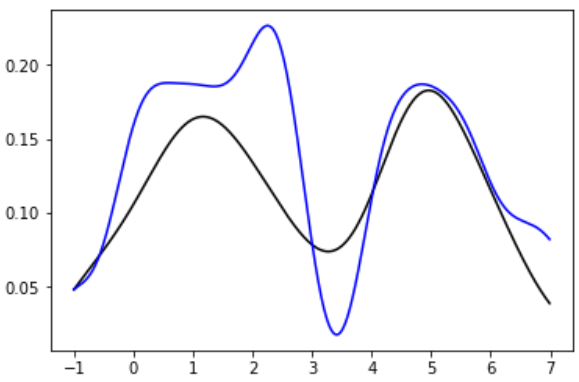
\includegraphics[width = 12cm, height = 6cm]{prva}
\end{figure}

\begin{figure}[!htb]
\centering
\caption{$\epsilon = 1$}
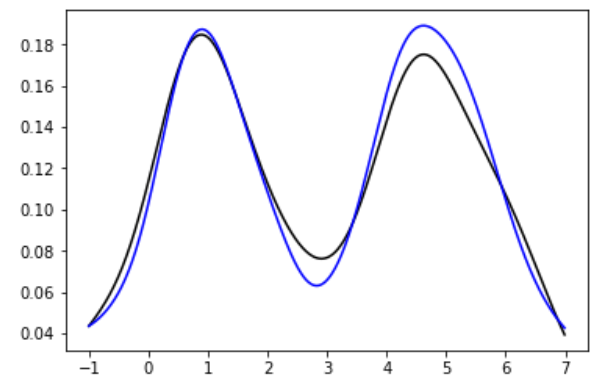
\includegraphics[width = 12cm, height = 6cm]{druga}
\end{figure}

\begin{figure}[!htb]
\centering
\caption{$\epsilon = 3$}
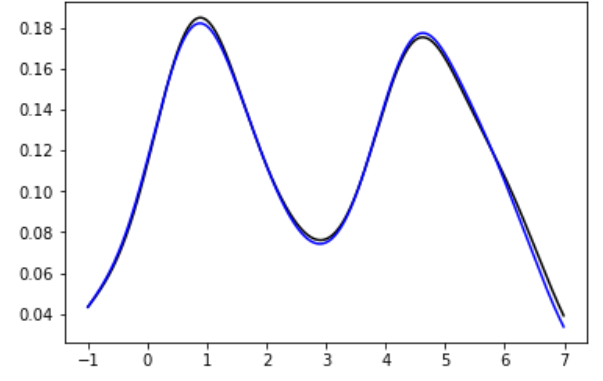
\includegraphics[width = 12cm, height = 6cm]{tretja}
\end{figure}

% seznam uporabljene literature
\begin{thebibliography}{99}

\bibitem{referenca-clanek}
N.~Holohan, D. J.~Leith in O.~Mason \emph{Numerical, categorical and functional data under the one roof}, Information Sciences \textbf{305} (2015) strani 256--268.
\bibitem{referenca-clanek}
R.~Hall, A.~Rinaldo in L.~Wasserman \emph{Differential Privacy for Functions and Functional Data}, Journal of M. L. Research \textbf{14} (2013) strani 703--727.
\bibitem{referenca-clanek}
Differential Privacy Team, Apple \emph{Learning with Privacy at Scale}, [ogled 22.07.2018], dostopno na \url{https://machinelearning.apple.com/docs/learning-with-privacy-at-scale/appledifferentialprivacysystem.pdf}.
\bibitem{referenca-clanek}
N.~Johnson, J. P.~Near in D.~Song \emph{Towards Practical Differential Privacy for SQL Queries
}, [ogled 22.07.2018], dostopno na \url{https://arxiv.org/abs/1706.09479}.
\bibitem{wiki}
\emph{Reproducing kernel Hilbert space}, v: Wikipedia: The Free Encyclopedia, [ogled 22.~7.~2018], dostopno na \url{https://en.wikipedia.org/wiki/Reproducing_kernel_Hilbert_space}.
\bibitem{wiki}
\emph{Differential Privacy}, v: Wikipedia: The Free Encyclopedia, [ogled 22.~7.~2018], dostopno na \url{https://en.wikipedia.org/wiki/Differential_Privacy}.
\bibitem{wiki}
\emph{Gaussian Process}, v: Wikipedia: The Free Encyclopedia, [ogled 22.~7.~2018], dostopno na \url{https://en.wikipedia.org/wiki/Gaussian_process}.
\bibitem{wiki}
\emph{Upper-tail inequality for standard normal distribution}, v: Mathematics Stack Exchange, [ogled 22.~7.~2018], dostopno na \url{https://math.stackexchange.com/questions/28751/proof-of-upper-tail-inequality-for-standard-normal-distribution/69417#69417}.
\bibitem{referenca-knjiga}
K.~Parthasarathy, \emph{Probability Measures on Metric Spaces}, AMS Chelsea Publishing, 2005 (ponatis).
\bibitem{referenca-knjiga}
P.~Billingsley, \emph{Probability and Measure}, Wiley--Interscience, 1995 (3. izdaja); dostopno tudi na naslovu \url{https://www.colorado.edu/amath/sites/default/files/attached-files/billingsley.pdf}.
\bibitem{referenca-clanek}
M.~Vidmar \emph{Dynkin ($\lambda$-) and $\pi$-systems; monotone classes of sets, and of
functions – with some examples of application (mainly of a
probabilistic flavor)}, [ogled 22.07.2018], dostopno na \url{https://www.fmf.uni-lj.si/~vidmarm/Dynkin_and_pi_systems.pdf} 
\bibitem{wiki}
\emph{Netflix IMDB data}, v: Wired, [ogled 22.~7.~2018], dostopno na \url{https://www.wired.com/2007/12/why-anonymous-data-sometimes-isnt/}.




\end{thebibliography}

\end{document}

